\chapter{How to Use the utdiss2 Package}
\index{How to Use the utdiss2 Package%
@\emph{How to Use the utdiss2 Package}}%

\section{Preamble}
\index{Preamble@\emph{Preamble}}%

The preamble of the document starts like this:
\begin{verbatim}
     \documentclass[12pt]{report}
     \usepackage{utdiss2}
\end{verbatim}
\index{commands!documentclass@\cn{documentclass}}%
\index{commands!usepackage@\cn{usepackage}}%

The first line declares ``\texttt{report}'' as the document 
class, 
\index{document class}%
with an option of 12pt for the character size, 
which is slightly greater that usual (the default is 10pt), but is
what the Office of the Graduate School (OGS) recommends.
You may include other options, as in any other \LaTeX{} document.

The second line loads the \texttt{utdiss2} package, 
\index{utdiss2 package@{\texttt{utdiss2} package}}%
which contains a set of commands intended to produce a document fulfilling
the official requirements for a doctoral dissertation or master's thesis or
report. Besides that, you may include other packages. 
For instance:
\begin{verbatim}
     \usepackage{amsmath,amsthm,amsfonts,amscd}
\end{verbatim}
for mathematical symbols, or,
\begin{verbatim}
     \usepackage{draftcopy}
\end{verbatim}
to have a large ``watermark'' across each page of your document that
says, ``DRAFT.''


The next few commands in the preamble are required.

\cn{author\{Craig William McCluskey\}}
\index{commands!author@\cn{author}}%
Replace my name in the command by your
full, official University name.  Make it combination of lower and uppercases.

\cn{address\{9905 Chukar Circle\bslash\bslash\ Austin, Texas 78758\}}
\index{commands!address@\cn{address}}%
Replace my address with your *permanent* (not local) address. Use
\texttt{\bslash\bslash} to separate address lines.

\cn{title\{Writing a Doctoral Dissertation with \cn{LaTeX\{\}} at
the University of Texas at Austin\} }
\index{commands!title@\cn{title}}%
Replace the name of this document
in this command by your dissertation title. If the title consists of more
than one line, it should be in inverted pyramid form. You may have to specify
the line breakings by \texttt{\bslash\bslash} commands.

\cn{supervisor[Isaac Newton]\{Johannes Kepler\} }
\index{commands!supervisor@\cn{supervisor}}%
This document has two supervisors listed. See the source file
(disstemplate.tex) for information on how to have only one supervisor.
This command can be broken across lines as it is in the source file and
as the \cn{committeemembers} command is shown below.

\begin{verbatim}
\committeemembers
        [Erwin Schr\"odinger]
        [Albert Einstein]
        [Charles Townes]
        {Arthur Schawlow}
\end{verbatim}
\index{commands!committeemembers@\cn{committeemembers}}%
This document shows four non-supervisor committee members. See the source
file (disstemplate.tex) for information on how to have a different number.

\cn{previousdegrees\{B.S.\} } Replace B.S. with your previous degree.

The next few commands in the preamble are optional.
\begin{verbatim}
%\graduationmonth{...}
%\graduationyear{...}
%\typist{...}
\end{verbatim}
Their use is documented in the source file.

At this point, if you are writing a master thesis or report
you must use the optional \cn{degree} and \cn{degreeabbr} commands
and specify
\index{master}
\index{master!master thesis}
\index{commands!masterthesis@\cn{masterthesis}}
\index{master!master report}
\index{commands!masterreport@\cn{masterreport}}
\begin{verbatim}
%\degree{MASTER OF ARTS}
%\degreeabbr{M.A.}
%\masterreport
%\masterthesis
\end{verbatim}
as documented in the source file. By default the document is formated
as a \emph{dissertation}%
\footnote{The command \cn{dissertation} is also provided for symmetry.}%
\index{commands!dissertation@\cn{dissertation}}


The default spacing for both text and quoted text is doublespaced.
That can be changed with the following self-explanatory commands: 
\begin{verbatim}
\oneandonehalfspacing 
\singlespacing
\oneandonehalfspacequote
\singlespacequote
\end{verbatim}
\index{commands!oneandonehalfspacing@\cn{oneandonehalfspacing}}%
\index{commands!singlespacing@\cn{singlespacing}}%
\index{commands!oneandonehalfspacequote@\cn{oneandonehalfspacequote}}%
\index{commands!singlespacequote@\cn{singlespacequote}}%

Some versions of LaTeX in combination with some types of printers
produce printed output that has incorrect vertical margins.
The command \cn{topmargin 0.125} is provided to allow easy adjustment
if it's needed.

If there are 10 or more sections, 10 or more subsections for a section,
etc., you need to make an adjustment to the Table of Contents with the
command \cn{longtocentry}.
\index{commands!longtocentry@\cn{longtocentry}}%
This command allocates the proper horizontal space for double-digit
numbers.


\section{Document}
\index{Document@\emph{Document}}%

Next comes the actual text. It could be a sequence of chapters divided
into sections, subsections, etc., all in the main file:
\begin{verbatim}
\chapter{...}     % The first chapter. The
                  % \chapter command is of the form
                  % \chapter[..]{..} or \chapter{..} where
    ... text ...  % [...] is the entry in table of contents
                  % and {...} is the chapter heading printed
                  % in the body of the document.
\section{...}     %
                  % IMPORTANT: If your chapter heading consists
                  % of more than one line, it will be auto-
    ... text ...  % matically broken into separate lines.
                  % If you don't like the way LaTeX breaks the
                  % chapter heading into lines, however, use
\section{...}     % `\newheadline' command to break lines.
                  % NEVER USE \\ IN SECTIONAL (E.G., CHAPTER,
    ... text ...  % SECTION, SUBSECTION, SUBSUBSECTION) HEADINGS!
                  %
\chapter{...}     % This is Chapter 2.
    ... text ...
\section{...}
    ... text...
\subsection{...}
    ... more text ...
\subsubsection{...}
    ... more text ...
\appendix         % The appendix begins here.
% \appendices     % If more than one appendix chapters,
                  % use \appendices instead of \appendix
\chapter{...}     % First appendix chapter, i.e., Appendix A.
\section{...}     % This is appendix section A.1.
    .................
\end{verbatim}
\index{commands!chapter@\cn{chapter}}%
\index{commands!section@\cn{section}}%
\index{commands!subsection@\cn{subsection}}%
\index{commands!appendix@\cn{appendix}}%
\index{commands!appendices@\cn{appendices}}%

Or, the chapters can be written in different files like this document
and be loaded by \cn{include} commands:
\begin{verbatim}
\chapter{Introduction}
\index{Introduction@\emph{Introduction}}%


This document deals with how to write a doctoral dissertation 
using \LaTeX{}, and how to use the \texttt{utdiss2} package. 
\index{utdiss2 package@{\texttt{utdiss2} package}}%

The latest version of this document/package can be obtained from
\url{http://www.ph.utexas.edu/~laser/craigs_stuff/LaTeX/}.\footnote{I
will be transferring this page to the Office of Graduate
Studies when I graduate. The new URL isn't defined yet, but I will
place a ``redirect'' at this URL to send your browser to the correct
location when the transition occurs.}
If your installation of LaTeX is missing any style files used in this
document (most likely with a \cn{usepackage\{package-name.sty\}}
command at the beginning of disstemplate.tex), take a look at the link
on this page to ``Frequently Requested Style Files'' or on the
Comprehensive TeX Archive Network, \url{http://www.ctan.org}.

In case of any confict between the requirements of the Office of Graduate
Studies and what this document says to do, the requirements of the Office
of Graduate Studies prevail.

\section{History of This Package}
\index{History of This Package@\emph{History of This Package}}%

In 1991 the \texttt{utdiss} package was written by Young U. Ryu 
\index{Young U. Ryu}%
in order to be used in the preamble of \LaTeX{} doctoral dissertation
files at the University of Texas at Austin. 
\index{University of Texas at Austin}%
Since then some changes have occured, the most important one
being the introduction of a new version of \LaTeX{} 
\index{LaTeX@{\LaTeX{}}}%
called \LaTeXe{}. 
\index{LaTeX2e@{\LaTeXe{}}}%

In order to partially adapt the utdiss package to this new version
of \LaTeX{}, Miguel Lerma introduced a few modifications in it,
and his document, \textit{How to Write a Doctoral Dissertation
with \LaTeX{}}, served as a test for it. His new package was
called \texttt{utdiss1}.
\index{utdiss1@\texttt{utdiss1}}%

With the significant changes in style introduced by the Graduate
School in the Spring of 2001, as well as  my need to write a
dissertation myself, I extended Miguel Lerma's package to meet
these new requirements. As in Miguel Lerma's case, this document
serves as a test for it, but it is, in addition, intended as a
template for others to use in writing their own dissertations.
The new package is called \texttt{utdiss2}.
\index{utdiss2@\texttt{utdiss2}}%

\section{Revised Philosophy for This Package}
\index{Revised Philosophy for This Package@\emph{Revised Philosophy
	for This Package}}%

Since the source file of this document is intended to be used by students
writing their own dissertations, this document does not display all of the
comments regarding usage of previous versions. It has, instead, transferred
these comments to their respective places in the source file so someone
editing their own copy of the source file to produce their own dissertation
will see the comments where they are needed. It may be helpful to print out
a copy of the source file along with the PostScript version of the document
so the two can be studied side-by-side.

\textbf{Note:} In spite of the effort to accommodate the package to
the requirements of the University, it is not possible to guarantee
that it will always work, and the author of the dissertation remains
responsible for checking that such requirements are actually fulfilled
by his/her final work. 

The standard caveat applies:

\begin{quote}
\index{guarantee}%
This template package is provided and licensed ``as is'' without warranty
of any kind, either expressed or implied, including, but not limited to,
the implied warranties of merchantability and fitness for a particular
purpose. Yadda, yadda, yadda, \ldots
\end{quote}

In case of any problem with the use of \texttt{utdiss2}, send me email
at \url{mccluskey@mail.utexas.edu}.

\chapter{Instructions for Preparing Dissertations, Theses, and Reports}
\index{Instructions for Preparing Dissertations, Theses, and Reports%
@\emph{Instructions for Preparing Dissertations, Theses, and Reports}}%

We are not going to look at the complete set of instructions contained
in \emph{Instructions for Preparation of Doctoral Dissertations and
Dissertation Abstracts} or \emph{Format For The Master's Thesis and Report}
which can be obtained from the Office of Graduate Studies (OGS)
\index{Office of Graduate Studies}%
or on their web page,
\index{Office of Graduate Studies web page}%
\url{http://www.utexas.edu/ogs}.
The doctoral Instructions I am using are dated March, 2001.
The master's Format I am using is dated May, 2001.

Here we will look at a few instructions related to the arrangement of the
dissertation, thesis, or report and a few other ``technical'' details,
providing some examples of common \LaTeX\ usage and some examples of
not-so-common \LaTeX\ usage.

The following are just a couple of tests for the ``quote''
and ``quotation'' environments. The following paragraph is a quote.
\begin{quote}
\index{quote}%
This template package is provided and licensed
``as is'' without warranty of any kind, either expressed or
implied, including, but not limited to, the implied warranties
of merchantability and fitness for a particular purpose.
\end{quote}
The following paragraph is a quotation.
\begin{quotation}
\index{quotation}%
This template package is provided and licensed
``as is'' without warranty of any kind, either expressed or
implied, including, but not limited to, the implied warranties
of merchantability and fitness for a particular purpose.
\end{quotation}

The OGS Instructions say prose quotations over four lines
should be indented on the left. The Doctoral Degree Evaluator says
the quote environment is the correct one to use.

\section{Arrangement of Dissertation}
\index{Arrangement of Dissertation@\emph{Arrangement of Dissertation}}%

Always remember that this ``fake'' dissertation 
\index{fake dissertation}%
is only intended to be a template for writing your own. Since the ultimate
responsibility of making sure your dissertation meets the Graduate School's
requirements, however, lies only with you, you \textbf{\textit{must}} get
the current \emph{Instructions for Preparation of Doctoral Dissertations and
Dissertation Abstracts} from the Office of Graduate Studies or their web
page and check everything yourself. If you don't, you may have a very
rude awakening from the Lynn Renegar, Doctoral Degree Evaluator (aka,
``The Ruler Lady'') at a most inopportune time.

Arrange your dissertation as follows (all sections are required 
unless said otherwise.

\begin{enumerate}

\item Fly Page 
\index{Fly Page}%
(blank protective page). This page is \textbf{not} counted in the numbering.
\textbf{Note:} This template does not insert a Fly Page; if you are printing
an official copy, you must manually insert a blank piece of paper on your own.
Electronic documents do not need a fly page.

\item Copyright Legend 
\index{Copyright Legend}%
(optional) - See OGS Instructions Sample Form A.
Begin counting \textbf{pretext} pages here, but \textbf{do not
place a number on this page.} 

\item Committee Certification of Approved Version.
\index{Committee Certification of Approved Version}%
See OGS Instructions Sample Form B. This page is included in the
pretext count, but there should be no page number on the page.

\item Title Page - 
\index{Title Page}%
See OGS Instructions Sample Form C.
This page is counted, but there should not be a page number on this page.

\item Dedication 
\index{Dedication}%
and/or Epigraph (optional). 
\index{Epigraph}%
Included in count, but not numbered.

\item Acknowledgments
\index{Acknowledgments}%
or Preface 
\index{Preface}%
(optional) - Begin showing \textbf{pretext} page numbers with \textbf{lower
case Roman numerals} at bottom of page.

\item Abstract 
\index{Abstract}%
(optional) - See OGS Instructions Sample Form D.

\item Table of contents -
\index{Table of contents}%
List ALL sections which follow it. There are too may different ways a table
of contents may be done for the OGS to give examples in their Instructions
booklet, but do be sure there is agreement between the major headings in
your text and their designations in the Table of Contents (fortunately \LaTeX{}
does this for you automatically). Please ask the Doctoral Degree Evaluator
for assistance if necessary.

\item List of Tables,
\index{List of Tables}%
List of Figures,
\index{List of figures}%
List of Illustrations, 
\index{List of Illustrations}% 
Nomenclature,
\index{Nomenclature}%
List of Supplemental Files (such as multimedia files)
(optional).

\item Text. 
\index{Text}%
The text should be divided into chapters, books or sections. The first page
is Arabic numeral \textbf{``1''}. All sections, \textbf{from the first page
of text through Vita,} should be numbered consecutively.

\item If you group all Tables, 
\index{Tables}%
Figures, 
\index{Figures}%
or Illustrations 
\index{Illustrations}%
in one place in your dissertation, the section should be placed 
here, immediately after the text and before any appendices 
(optional).

\item Appendix or Appendices 
\index{Appendix}%
\index{Appendices}%
(optional).

\item Glossary 
\index{Glossary}%
(optional) - this section may be placed either here or after the Table
of Contents, in the area with List of Tables, List of Figures...

\item Bibliography
\index{Bibliography}%
- consult your supervisor about which recognized style to use.

\item Index
\index{Index}%
(optional).

\item Vita -
\index{Vita}%
This should be a brief biographical sketch of the author. List in the
Table of Contents. See OGS Instructions Sample Form E.


\end{enumerate}


\section{Other Requirements}
\index{Other Requirements@\emph{Other Requirements}}%


\subsection{Margins}
\index{Margins@\emph{Margins}}%

The dissertation, after printing, should have left and top margins of
1~1/2 inches, and the right and bottom margins should be 1~1/4 inches.
These margins should be consistent throughout the dissertation - including
all pages in the appendix. \textbf{All page numbers must be \textit{at
least} one inch from the edges of the page}. Headers are rarely used in
dissertations; if you are considering using them, check with the Doctoral
Degree Evaluator first to be sure they will be accepted.


\subsection{Spacing and Page Arrangement}
\index{Spacing and Page Arrangement@\emph{Spacing and Page Arrangement}}
\index{Spacing}%
\index{Page Arrangement}%

The document should be double-spaced or space-and-a-half. 
Exceptions to double-spacing are: the Table of Contents, Lists of Tables, 
Tables, Figures, Graphs, Captions, Footnotes, Endnotes, 
Appendices, Glossary, Bibliography and Index; these may 
be single-spaced. Paragraph indentations are usually five to ten 
spaces. Prose quotations over four lines should be in 
block quote (double or single spaced, indented on the left). 
Do not use quotation marks if the quotation is indented except for
quotations within the block quote. Please refer to a style manual for
more detailed instructions.

Be sure that each new chapter or major section (i.e., Appendix, Bibliography,
Vita) begins on a new page.

\section{Master's Theses and Reports}

Always remember that this ``fake'' thesis or report 
\index{fake thesis or report}%
--- assuming you have followed the instructions in the next chapter about
how to format it as such --- is only intended to be a template for writing
your own. Since the ultimate responsibility of making sure your thesis or
report meets the Graduate School's requirements, however, lies only with
you, you \textbf{\textit{must}} get the current \emph{Format For The
Master's Thesis and Report} from the Office of Graduate Studies or their web
page and check everything yourself. If you don't, you may have a very
rude awakening from the Mike Feissli, Master's Degree Evaluator at a most
inopportune time.

That said, the formatting requirements for Dissertations and Reports and
Theses are very similar. They are, however, \textbf{\textit{not}} identical.
The primary differences are in the ordering of the title and signature
pages and where the optional index is inserted. For Master's Theses
and Reports, the Title Page must be in front of the Signature Page. For
Master's Theses and Reports, \textbf{\textit{nothing}} is permitted to
come between the bibliography and the vita; the index, if used, must be
before the bibliography. If you want to use an index, talk with Mike
Feissli before your deadline to verify that its inclusion is
acceptable. The index can be removed by commenting out one line with a
percent sign, if necessary, for producing the ``official'' copy of your
thesis or report, and then inserted for copies for your advisor and
you by removing the percent sign.


\chapter{How to Use the utdiss2 Package}
\index{How to Use the utdiss2 Package%
@\emph{How to Use the utdiss2 Package}}%

\section{Preamble}
\index{Preamble@\emph{Preamble}}%

The preamble of the document starts like this:
\begin{verbatim}
     \documentclass[12pt]{report}
     \usepackage{utdiss2}
\end{verbatim}
\index{commands!documentclass@\cn{documentclass}}%
\index{commands!usepackage@\cn{usepackage}}%

The first line declares ``\texttt{report}'' as the document 
class, 
\index{document class}%
with an option of 12pt for the character size, 
which is slightly greater that usual (the default is 10pt), but is
what the Office of the Graduate School (OGS) recommends.
You may include other options, as in any other \LaTeX{} document.

The second line loads the \texttt{utdiss2} package, 
\index{utdiss2 package@{\texttt{utdiss2} package}}%
which contains a set of commands intended to produce a document fulfilling
the official requirements for a doctoral dissertation or master's thesis or
report. Besides that, you may include other packages. 
For instance:
\begin{verbatim}
     \usepackage{amsmath,amsthm,amsfonts,amscd}
\end{verbatim}
for mathematical symbols, or,
\begin{verbatim}
     \usepackage{draftcopy}
\end{verbatim}
to have a large ``watermark'' across each page of your document that
says, ``DRAFT.''


The next few commands in the preamble are required.

\cn{author\{Craig William McCluskey\}}
\index{commands!author@\cn{author}}%
Replace my name in the command by your
full, official University name.  Make it combination of lower and uppercases.

\cn{address\{9905 Chukar Circle\bslash\bslash\ Austin, Texas 78758\}}
\index{commands!address@\cn{address}}%
Replace my address with your *permanent* (not local) address. Use
\texttt{\bslash\bslash} to separate address lines.

\cn{title\{Writing a Doctoral Dissertation with \cn{LaTeX\{\}} at
the University of Texas at Austin\} }
\index{commands!title@\cn{title}}%
Replace the name of this document
in this command by your dissertation title. If the title consists of more
than one line, it should be in inverted pyramid form. You may have to specify
the line breakings by \texttt{\bslash\bslash} commands.

\cn{supervisor[Isaac Newton]\{Johannes Kepler\} }
\index{commands!supervisor@\cn{supervisor}}%
This document has two supervisors listed. See the source file
(disstemplate.tex) for information on how to have only one supervisor.
This command can be broken across lines as it is in the source file and
as the \cn{committeemembers} command is shown below.

\begin{verbatim}
\committeemembers
        [Erwin Schr\"odinger]
        [Albert Einstein]
        [Charles Townes]
        {Arthur Schawlow}
\end{verbatim}
\index{commands!committeemembers@\cn{committeemembers}}%
This document shows four non-supervisor committee members. See the source
file (disstemplate.tex) for information on how to have a different number.

\cn{previousdegrees\{B.S.\} } Replace B.S. with your previous degree.

The next few commands in the preamble are optional.
\begin{verbatim}
%\graduationmonth{...}
%\graduationyear{...}
%\typist{...}
\end{verbatim}
Their use is documented in the source file.

At this point, if you are writing a master thesis or report
you must use the optional \cn{degree} and \cn{degreeabbr} commands
and specify
\index{master}
\index{master!master thesis}
\index{commands!masterthesis@\cn{masterthesis}}
\index{master!master report}
\index{commands!masterreport@\cn{masterreport}}
\begin{verbatim}
%\degree{MASTER OF ARTS}
%\degreeabbr{M.A.}
%\masterreport
%\masterthesis
\end{verbatim}
as documented in the source file. By default the document is formated
as a \emph{dissertation}%
\footnote{The command \cn{dissertation} is also provided for symmetry.}%
\index{commands!dissertation@\cn{dissertation}}


The default spacing for both text and quoted text is doublespaced.
That can be changed with the following self-explanatory commands: 
\begin{verbatim}
\oneandonehalfspacing 
\singlespacing
\oneandonehalfspacequote
\singlespacequote
\end{verbatim}
\index{commands!oneandonehalfspacing@\cn{oneandonehalfspacing}}%
\index{commands!singlespacing@\cn{singlespacing}}%
\index{commands!oneandonehalfspacequote@\cn{oneandonehalfspacequote}}%
\index{commands!singlespacequote@\cn{singlespacequote}}%

Some versions of LaTeX in combination with some types of printers
produce printed output that has incorrect vertical margins.
The command \cn{topmargin 0.125} is provided to allow easy adjustment
if it's needed.

If there are 10 or more sections, 10 or more subsections for a section,
etc., you need to make an adjustment to the Table of Contents with the
command \cn{longtocentry}.
\index{commands!longtocentry@\cn{longtocentry}}%
This command allocates the proper horizontal space for double-digit
numbers.


\section{Document}
\index{Document@\emph{Document}}%

Next comes the actual text. It could be a sequence of chapters divided
into sections, subsections, etc., all in the main file:
\begin{verbatim}
\chapter{...}     % The first chapter. The
                  % \chapter command is of the form
                  % \chapter[..]{..} or \chapter{..} where
    ... text ...  % [...] is the entry in table of contents
                  % and {...} is the chapter heading printed
                  % in the body of the document.
\section{...}     %
                  % IMPORTANT: If your chapter heading consists
                  % of more than one line, it will be auto-
    ... text ...  % matically broken into separate lines.
                  % If you don't like the way LaTeX breaks the
                  % chapter heading into lines, however, use
\section{...}     % `\newheadline' command to break lines.
                  % NEVER USE \\ IN SECTIONAL (E.G., CHAPTER,
    ... text ...  % SECTION, SUBSECTION, SUBSUBSECTION) HEADINGS!
                  %
\chapter{...}     % This is Chapter 2.
    ... text ...
\section{...}
    ... text...
\subsection{...}
    ... more text ...
\subsubsection{...}
    ... more text ...
\appendix         % The appendix begins here.
% \appendices     % If more than one appendix chapters,
                  % use \appendices instead of \appendix
\chapter{...}     % First appendix chapter, i.e., Appendix A.
\section{...}     % This is appendix section A.1.
    .................
\end{verbatim}
\index{commands!chapter@\cn{chapter}}%
\index{commands!section@\cn{section}}%
\index{commands!subsection@\cn{subsection}}%
\index{commands!appendix@\cn{appendix}}%
\index{commands!appendices@\cn{appendices}}%

Or, the chapters can be written in different files like this document
and be loaded by \cn{include} commands:
\begin{verbatim}
\chapter{Introduction}
\index{Introduction@\emph{Introduction}}%


This document deals with how to write a doctoral dissertation 
using \LaTeX{}, and how to use the \texttt{utdiss2} package. 
\index{utdiss2 package@{\texttt{utdiss2} package}}%

The latest version of this document/package can be obtained from
\url{http://www.ph.utexas.edu/~laser/craigs_stuff/LaTeX/}.\footnote{I
will be transferring this page to the Office of Graduate
Studies when I graduate. The new URL isn't defined yet, but I will
place a ``redirect'' at this URL to send your browser to the correct
location when the transition occurs.}
If your installation of LaTeX is missing any style files used in this
document (most likely with a \cn{usepackage\{package-name.sty\}}
command at the beginning of disstemplate.tex), take a look at the link
on this page to ``Frequently Requested Style Files'' or on the
Comprehensive TeX Archive Network, \url{http://www.ctan.org}.

In case of any confict between the requirements of the Office of Graduate
Studies and what this document says to do, the requirements of the Office
of Graduate Studies prevail.

\section{History of This Package}
\index{History of This Package@\emph{History of This Package}}%

In 1991 the \texttt{utdiss} package was written by Young U. Ryu 
\index{Young U. Ryu}%
in order to be used in the preamble of \LaTeX{} doctoral dissertation
files at the University of Texas at Austin. 
\index{University of Texas at Austin}%
Since then some changes have occured, the most important one
being the introduction of a new version of \LaTeX{} 
\index{LaTeX@{\LaTeX{}}}%
called \LaTeXe{}. 
\index{LaTeX2e@{\LaTeXe{}}}%

In order to partially adapt the utdiss package to this new version
of \LaTeX{}, Miguel Lerma introduced a few modifications in it,
and his document, \textit{How to Write a Doctoral Dissertation
with \LaTeX{}}, served as a test for it. His new package was
called \texttt{utdiss1}.
\index{utdiss1@\texttt{utdiss1}}%

With the significant changes in style introduced by the Graduate
School in the Spring of 2001, as well as  my need to write a
dissertation myself, I extended Miguel Lerma's package to meet
these new requirements. As in Miguel Lerma's case, this document
serves as a test for it, but it is, in addition, intended as a
template for others to use in writing their own dissertations.
The new package is called \texttt{utdiss2}.
\index{utdiss2@\texttt{utdiss2}}%

\section{Revised Philosophy for This Package}
\index{Revised Philosophy for This Package@\emph{Revised Philosophy
	for This Package}}%

Since the source file of this document is intended to be used by students
writing their own dissertations, this document does not display all of the
comments regarding usage of previous versions. It has, instead, transferred
these comments to their respective places in the source file so someone
editing their own copy of the source file to produce their own dissertation
will see the comments where they are needed. It may be helpful to print out
a copy of the source file along with the PostScript version of the document
so the two can be studied side-by-side.

\textbf{Note:} In spite of the effort to accommodate the package to
the requirements of the University, it is not possible to guarantee
that it will always work, and the author of the dissertation remains
responsible for checking that such requirements are actually fulfilled
by his/her final work. 

The standard caveat applies:

\begin{quote}
\index{guarantee}%
This template package is provided and licensed ``as is'' without warranty
of any kind, either expressed or implied, including, but not limited to,
the implied warranties of merchantability and fitness for a particular
purpose. Yadda, yadda, yadda, \ldots
\end{quote}

In case of any problem with the use of \texttt{utdiss2}, send me email
at \url{mccluskey@mail.utexas.edu}.

\chapter{Instructions for Preparing Dissertations, Theses, and Reports}
\index{Instructions for Preparing Dissertations, Theses, and Reports%
@\emph{Instructions for Preparing Dissertations, Theses, and Reports}}%

We are not going to look at the complete set of instructions contained
in \emph{Instructions for Preparation of Doctoral Dissertations and
Dissertation Abstracts} or \emph{Format For The Master's Thesis and Report}
which can be obtained from the Office of Graduate Studies (OGS)
\index{Office of Graduate Studies}%
or on their web page,
\index{Office of Graduate Studies web page}%
\url{http://www.utexas.edu/ogs}.
The doctoral Instructions I am using are dated March, 2001.
The master's Format I am using is dated May, 2001.

Here we will look at a few instructions related to the arrangement of the
dissertation, thesis, or report and a few other ``technical'' details,
providing some examples of common \LaTeX\ usage and some examples of
not-so-common \LaTeX\ usage.

The following are just a couple of tests for the ``quote''
and ``quotation'' environments. The following paragraph is a quote.
\begin{quote}
\index{quote}%
This template package is provided and licensed
``as is'' without warranty of any kind, either expressed or
implied, including, but not limited to, the implied warranties
of merchantability and fitness for a particular purpose.
\end{quote}
The following paragraph is a quotation.
\begin{quotation}
\index{quotation}%
This template package is provided and licensed
``as is'' without warranty of any kind, either expressed or
implied, including, but not limited to, the implied warranties
of merchantability and fitness for a particular purpose.
\end{quotation}

The OGS Instructions say prose quotations over four lines
should be indented on the left. The Doctoral Degree Evaluator says
the quote environment is the correct one to use.

\section{Arrangement of Dissertation}
\index{Arrangement of Dissertation@\emph{Arrangement of Dissertation}}%

Always remember that this ``fake'' dissertation 
\index{fake dissertation}%
is only intended to be a template for writing your own. Since the ultimate
responsibility of making sure your dissertation meets the Graduate School's
requirements, however, lies only with you, you \textbf{\textit{must}} get
the current \emph{Instructions for Preparation of Doctoral Dissertations and
Dissertation Abstracts} from the Office of Graduate Studies or their web
page and check everything yourself. If you don't, you may have a very
rude awakening from the Lynn Renegar, Doctoral Degree Evaluator (aka,
``The Ruler Lady'') at a most inopportune time.

Arrange your dissertation as follows (all sections are required 
unless said otherwise.

\begin{enumerate}

\item Fly Page 
\index{Fly Page}%
(blank protective page). This page is \textbf{not} counted in the numbering.
\textbf{Note:} This template does not insert a Fly Page; if you are printing
an official copy, you must manually insert a blank piece of paper on your own.
Electronic documents do not need a fly page.

\item Copyright Legend 
\index{Copyright Legend}%
(optional) - See OGS Instructions Sample Form A.
Begin counting \textbf{pretext} pages here, but \textbf{do not
place a number on this page.} 

\item Committee Certification of Approved Version.
\index{Committee Certification of Approved Version}%
See OGS Instructions Sample Form B. This page is included in the
pretext count, but there should be no page number on the page.

\item Title Page - 
\index{Title Page}%
See OGS Instructions Sample Form C.
This page is counted, but there should not be a page number on this page.

\item Dedication 
\index{Dedication}%
and/or Epigraph (optional). 
\index{Epigraph}%
Included in count, but not numbered.

\item Acknowledgments
\index{Acknowledgments}%
or Preface 
\index{Preface}%
(optional) - Begin showing \textbf{pretext} page numbers with \textbf{lower
case Roman numerals} at bottom of page.

\item Abstract 
\index{Abstract}%
(optional) - See OGS Instructions Sample Form D.

\item Table of contents -
\index{Table of contents}%
List ALL sections which follow it. There are too may different ways a table
of contents may be done for the OGS to give examples in their Instructions
booklet, but do be sure there is agreement between the major headings in
your text and their designations in the Table of Contents (fortunately \LaTeX{}
does this for you automatically). Please ask the Doctoral Degree Evaluator
for assistance if necessary.

\item List of Tables,
\index{List of Tables}%
List of Figures,
\index{List of figures}%
List of Illustrations, 
\index{List of Illustrations}% 
Nomenclature,
\index{Nomenclature}%
List of Supplemental Files (such as multimedia files)
(optional).

\item Text. 
\index{Text}%
The text should be divided into chapters, books or sections. The first page
is Arabic numeral \textbf{``1''}. All sections, \textbf{from the first page
of text through Vita,} should be numbered consecutively.

\item If you group all Tables, 
\index{Tables}%
Figures, 
\index{Figures}%
or Illustrations 
\index{Illustrations}%
in one place in your dissertation, the section should be placed 
here, immediately after the text and before any appendices 
(optional).

\item Appendix or Appendices 
\index{Appendix}%
\index{Appendices}%
(optional).

\item Glossary 
\index{Glossary}%
(optional) - this section may be placed either here or after the Table
of Contents, in the area with List of Tables, List of Figures...

\item Bibliography
\index{Bibliography}%
- consult your supervisor about which recognized style to use.

\item Index
\index{Index}%
(optional).

\item Vita -
\index{Vita}%
This should be a brief biographical sketch of the author. List in the
Table of Contents. See OGS Instructions Sample Form E.


\end{enumerate}


\section{Other Requirements}
\index{Other Requirements@\emph{Other Requirements}}%


\subsection{Margins}
\index{Margins@\emph{Margins}}%

The dissertation, after printing, should have left and top margins of
1~1/2 inches, and the right and bottom margins should be 1~1/4 inches.
These margins should be consistent throughout the dissertation - including
all pages in the appendix. \textbf{All page numbers must be \textit{at
least} one inch from the edges of the page}. Headers are rarely used in
dissertations; if you are considering using them, check with the Doctoral
Degree Evaluator first to be sure they will be accepted.


\subsection{Spacing and Page Arrangement}
\index{Spacing and Page Arrangement@\emph{Spacing and Page Arrangement}}
\index{Spacing}%
\index{Page Arrangement}%

The document should be double-spaced or space-and-a-half. 
Exceptions to double-spacing are: the Table of Contents, Lists of Tables, 
Tables, Figures, Graphs, Captions, Footnotes, Endnotes, 
Appendices, Glossary, Bibliography and Index; these may 
be single-spaced. Paragraph indentations are usually five to ten 
spaces. Prose quotations over four lines should be in 
block quote (double or single spaced, indented on the left). 
Do not use quotation marks if the quotation is indented except for
quotations within the block quote. Please refer to a style manual for
more detailed instructions.

Be sure that each new chapter or major section (i.e., Appendix, Bibliography,
Vita) begins on a new page.

\section{Master's Theses and Reports}

Always remember that this ``fake'' thesis or report 
\index{fake thesis or report}%
--- assuming you have followed the instructions in the next chapter about
how to format it as such --- is only intended to be a template for writing
your own. Since the ultimate responsibility of making sure your thesis or
report meets the Graduate School's requirements, however, lies only with
you, you \textbf{\textit{must}} get the current \emph{Format For The
Master's Thesis and Report} from the Office of Graduate Studies or their web
page and check everything yourself. If you don't, you may have a very
rude awakening from the Mike Feissli, Master's Degree Evaluator at a most
inopportune time.

That said, the formatting requirements for Dissertations and Reports and
Theses are very similar. They are, however, \textbf{\textit{not}} identical.
The primary differences are in the ordering of the title and signature
pages and where the optional index is inserted. For Master's Theses
and Reports, the Title Page must be in front of the Signature Page. For
Master's Theses and Reports, \textbf{\textit{nothing}} is permitted to
come between the bibliography and the vita; the index, if used, must be
before the bibliography. If you want to use an index, talk with Mike
Feissli before your deadline to verify that its inclusion is
acceptable. The index can be removed by commenting out one line with a
percent sign, if necessary, for producing the ``official'' copy of your
thesis or report, and then inserted for copies for your advisor and
you by removing the percent sign.


\chapter{How to Use the utdiss2 Package}
\index{How to Use the utdiss2 Package%
@\emph{How to Use the utdiss2 Package}}%

\section{Preamble}
\index{Preamble@\emph{Preamble}}%

The preamble of the document starts like this:
\begin{verbatim}
     \documentclass[12pt]{report}
     \usepackage{utdiss2}
\end{verbatim}
\index{commands!documentclass@\cn{documentclass}}%
\index{commands!usepackage@\cn{usepackage}}%

The first line declares ``\texttt{report}'' as the document 
class, 
\index{document class}%
with an option of 12pt for the character size, 
which is slightly greater that usual (the default is 10pt), but is
what the Office of the Graduate School (OGS) recommends.
You may include other options, as in any other \LaTeX{} document.

The second line loads the \texttt{utdiss2} package, 
\index{utdiss2 package@{\texttt{utdiss2} package}}%
which contains a set of commands intended to produce a document fulfilling
the official requirements for a doctoral dissertation or master's thesis or
report. Besides that, you may include other packages. 
For instance:
\begin{verbatim}
     \usepackage{amsmath,amsthm,amsfonts,amscd}
\end{verbatim}
for mathematical symbols, or,
\begin{verbatim}
     \usepackage{draftcopy}
\end{verbatim}
to have a large ``watermark'' across each page of your document that
says, ``DRAFT.''


The next few commands in the preamble are required.

\cn{author\{Craig William McCluskey\}}
\index{commands!author@\cn{author}}%
Replace my name in the command by your
full, official University name.  Make it combination of lower and uppercases.

\cn{address\{9905 Chukar Circle\bslash\bslash\ Austin, Texas 78758\}}
\index{commands!address@\cn{address}}%
Replace my address with your *permanent* (not local) address. Use
\texttt{\bslash\bslash} to separate address lines.

\cn{title\{Writing a Doctoral Dissertation with \cn{LaTeX\{\}} at
the University of Texas at Austin\} }
\index{commands!title@\cn{title}}%
Replace the name of this document
in this command by your dissertation title. If the title consists of more
than one line, it should be in inverted pyramid form. You may have to specify
the line breakings by \texttt{\bslash\bslash} commands.

\cn{supervisor[Isaac Newton]\{Johannes Kepler\} }
\index{commands!supervisor@\cn{supervisor}}%
This document has two supervisors listed. See the source file
(disstemplate.tex) for information on how to have only one supervisor.
This command can be broken across lines as it is in the source file and
as the \cn{committeemembers} command is shown below.

\begin{verbatim}
\committeemembers
        [Erwin Schr\"odinger]
        [Albert Einstein]
        [Charles Townes]
        {Arthur Schawlow}
\end{verbatim}
\index{commands!committeemembers@\cn{committeemembers}}%
This document shows four non-supervisor committee members. See the source
file (disstemplate.tex) for information on how to have a different number.

\cn{previousdegrees\{B.S.\} } Replace B.S. with your previous degree.

The next few commands in the preamble are optional.
\begin{verbatim}
%\graduationmonth{...}
%\graduationyear{...}
%\typist{...}
\end{verbatim}
Their use is documented in the source file.

At this point, if you are writing a master thesis or report
you must use the optional \cn{degree} and \cn{degreeabbr} commands
and specify
\index{master}
\index{master!master thesis}
\index{commands!masterthesis@\cn{masterthesis}}
\index{master!master report}
\index{commands!masterreport@\cn{masterreport}}
\begin{verbatim}
%\degree{MASTER OF ARTS}
%\degreeabbr{M.A.}
%\masterreport
%\masterthesis
\end{verbatim}
as documented in the source file. By default the document is formated
as a \emph{dissertation}%
\footnote{The command \cn{dissertation} is also provided for symmetry.}%
\index{commands!dissertation@\cn{dissertation}}


The default spacing for both text and quoted text is doublespaced.
That can be changed with the following self-explanatory commands: 
\begin{verbatim}
\oneandonehalfspacing 
\singlespacing
\oneandonehalfspacequote
\singlespacequote
\end{verbatim}
\index{commands!oneandonehalfspacing@\cn{oneandonehalfspacing}}%
\index{commands!singlespacing@\cn{singlespacing}}%
\index{commands!oneandonehalfspacequote@\cn{oneandonehalfspacequote}}%
\index{commands!singlespacequote@\cn{singlespacequote}}%

Some versions of LaTeX in combination with some types of printers
produce printed output that has incorrect vertical margins.
The command \cn{topmargin 0.125} is provided to allow easy adjustment
if it's needed.

If there are 10 or more sections, 10 or more subsections for a section,
etc., you need to make an adjustment to the Table of Contents with the
command \cn{longtocentry}.
\index{commands!longtocentry@\cn{longtocentry}}%
This command allocates the proper horizontal space for double-digit
numbers.


\section{Document}
\index{Document@\emph{Document}}%

Next comes the actual text. It could be a sequence of chapters divided
into sections, subsections, etc., all in the main file:
\begin{verbatim}
\chapter{...}     % The first chapter. The
                  % \chapter command is of the form
                  % \chapter[..]{..} or \chapter{..} where
    ... text ...  % [...] is the entry in table of contents
                  % and {...} is the chapter heading printed
                  % in the body of the document.
\section{...}     %
                  % IMPORTANT: If your chapter heading consists
                  % of more than one line, it will be auto-
    ... text ...  % matically broken into separate lines.
                  % If you don't like the way LaTeX breaks the
                  % chapter heading into lines, however, use
\section{...}     % `\newheadline' command to break lines.
                  % NEVER USE \\ IN SECTIONAL (E.G., CHAPTER,
    ... text ...  % SECTION, SUBSECTION, SUBSUBSECTION) HEADINGS!
                  %
\chapter{...}     % This is Chapter 2.
    ... text ...
\section{...}
    ... text...
\subsection{...}
    ... more text ...
\subsubsection{...}
    ... more text ...
\appendix         % The appendix begins here.
% \appendices     % If more than one appendix chapters,
                  % use \appendices instead of \appendix
\chapter{...}     % First appendix chapter, i.e., Appendix A.
\section{...}     % This is appendix section A.1.
    .................
\end{verbatim}
\index{commands!chapter@\cn{chapter}}%
\index{commands!section@\cn{section}}%
\index{commands!subsection@\cn{subsection}}%
\index{commands!appendix@\cn{appendix}}%
\index{commands!appendices@\cn{appendices}}%

Or, the chapters can be written in different files like this document
and be loaded by \cn{include} commands:
\begin{verbatim}
\chapter{Introduction}
\index{Introduction@\emph{Introduction}}%


This document deals with how to write a doctoral dissertation 
using \LaTeX{}, and how to use the \texttt{utdiss2} package. 
\index{utdiss2 package@{\texttt{utdiss2} package}}%

The latest version of this document/package can be obtained from
\url{http://www.ph.utexas.edu/~laser/craigs_stuff/LaTeX/}.\footnote{I
will be transferring this page to the Office of Graduate
Studies when I graduate. The new URL isn't defined yet, but I will
place a ``redirect'' at this URL to send your browser to the correct
location when the transition occurs.}
If your installation of LaTeX is missing any style files used in this
document (most likely with a \cn{usepackage\{package-name.sty\}}
command at the beginning of disstemplate.tex), take a look at the link
on this page to ``Frequently Requested Style Files'' or on the
Comprehensive TeX Archive Network, \url{http://www.ctan.org}.

In case of any confict between the requirements of the Office of Graduate
Studies and what this document says to do, the requirements of the Office
of Graduate Studies prevail.

\section{History of This Package}
\index{History of This Package@\emph{History of This Package}}%

In 1991 the \texttt{utdiss} package was written by Young U. Ryu 
\index{Young U. Ryu}%
in order to be used in the preamble of \LaTeX{} doctoral dissertation
files at the University of Texas at Austin. 
\index{University of Texas at Austin}%
Since then some changes have occured, the most important one
being the introduction of a new version of \LaTeX{} 
\index{LaTeX@{\LaTeX{}}}%
called \LaTeXe{}. 
\index{LaTeX2e@{\LaTeXe{}}}%

In order to partially adapt the utdiss package to this new version
of \LaTeX{}, Miguel Lerma introduced a few modifications in it,
and his document, \textit{How to Write a Doctoral Dissertation
with \LaTeX{}}, served as a test for it. His new package was
called \texttt{utdiss1}.
\index{utdiss1@\texttt{utdiss1}}%

With the significant changes in style introduced by the Graduate
School in the Spring of 2001, as well as  my need to write a
dissertation myself, I extended Miguel Lerma's package to meet
these new requirements. As in Miguel Lerma's case, this document
serves as a test for it, but it is, in addition, intended as a
template for others to use in writing their own dissertations.
The new package is called \texttt{utdiss2}.
\index{utdiss2@\texttt{utdiss2}}%

\section{Revised Philosophy for This Package}
\index{Revised Philosophy for This Package@\emph{Revised Philosophy
	for This Package}}%

Since the source file of this document is intended to be used by students
writing their own dissertations, this document does not display all of the
comments regarding usage of previous versions. It has, instead, transferred
these comments to their respective places in the source file so someone
editing their own copy of the source file to produce their own dissertation
will see the comments where they are needed. It may be helpful to print out
a copy of the source file along with the PostScript version of the document
so the two can be studied side-by-side.

\textbf{Note:} In spite of the effort to accommodate the package to
the requirements of the University, it is not possible to guarantee
that it will always work, and the author of the dissertation remains
responsible for checking that such requirements are actually fulfilled
by his/her final work. 

The standard caveat applies:

\begin{quote}
\index{guarantee}%
This template package is provided and licensed ``as is'' without warranty
of any kind, either expressed or implied, including, but not limited to,
the implied warranties of merchantability and fitness for a particular
purpose. Yadda, yadda, yadda, \ldots
\end{quote}

In case of any problem with the use of \texttt{utdiss2}, send me email
at \url{mccluskey@mail.utexas.edu}.

\chapter{Instructions for Preparing Dissertations, Theses, and Reports}
\index{Instructions for Preparing Dissertations, Theses, and Reports%
@\emph{Instructions for Preparing Dissertations, Theses, and Reports}}%

We are not going to look at the complete set of instructions contained
in \emph{Instructions for Preparation of Doctoral Dissertations and
Dissertation Abstracts} or \emph{Format For The Master's Thesis and Report}
which can be obtained from the Office of Graduate Studies (OGS)
\index{Office of Graduate Studies}%
or on their web page,
\index{Office of Graduate Studies web page}%
\url{http://www.utexas.edu/ogs}.
The doctoral Instructions I am using are dated March, 2001.
The master's Format I am using is dated May, 2001.

Here we will look at a few instructions related to the arrangement of the
dissertation, thesis, or report and a few other ``technical'' details,
providing some examples of common \LaTeX\ usage and some examples of
not-so-common \LaTeX\ usage.

The following are just a couple of tests for the ``quote''
and ``quotation'' environments. The following paragraph is a quote.
\begin{quote}
\index{quote}%
This template package is provided and licensed
``as is'' without warranty of any kind, either expressed or
implied, including, but not limited to, the implied warranties
of merchantability and fitness for a particular purpose.
\end{quote}
The following paragraph is a quotation.
\begin{quotation}
\index{quotation}%
This template package is provided and licensed
``as is'' without warranty of any kind, either expressed or
implied, including, but not limited to, the implied warranties
of merchantability and fitness for a particular purpose.
\end{quotation}

The OGS Instructions say prose quotations over four lines
should be indented on the left. The Doctoral Degree Evaluator says
the quote environment is the correct one to use.

\section{Arrangement of Dissertation}
\index{Arrangement of Dissertation@\emph{Arrangement of Dissertation}}%

Always remember that this ``fake'' dissertation 
\index{fake dissertation}%
is only intended to be a template for writing your own. Since the ultimate
responsibility of making sure your dissertation meets the Graduate School's
requirements, however, lies only with you, you \textbf{\textit{must}} get
the current \emph{Instructions for Preparation of Doctoral Dissertations and
Dissertation Abstracts} from the Office of Graduate Studies or their web
page and check everything yourself. If you don't, you may have a very
rude awakening from the Lynn Renegar, Doctoral Degree Evaluator (aka,
``The Ruler Lady'') at a most inopportune time.

Arrange your dissertation as follows (all sections are required 
unless said otherwise.

\begin{enumerate}

\item Fly Page 
\index{Fly Page}%
(blank protective page). This page is \textbf{not} counted in the numbering.
\textbf{Note:} This template does not insert a Fly Page; if you are printing
an official copy, you must manually insert a blank piece of paper on your own.
Electronic documents do not need a fly page.

\item Copyright Legend 
\index{Copyright Legend}%
(optional) - See OGS Instructions Sample Form A.
Begin counting \textbf{pretext} pages here, but \textbf{do not
place a number on this page.} 

\item Committee Certification of Approved Version.
\index{Committee Certification of Approved Version}%
See OGS Instructions Sample Form B. This page is included in the
pretext count, but there should be no page number on the page.

\item Title Page - 
\index{Title Page}%
See OGS Instructions Sample Form C.
This page is counted, but there should not be a page number on this page.

\item Dedication 
\index{Dedication}%
and/or Epigraph (optional). 
\index{Epigraph}%
Included in count, but not numbered.

\item Acknowledgments
\index{Acknowledgments}%
or Preface 
\index{Preface}%
(optional) - Begin showing \textbf{pretext} page numbers with \textbf{lower
case Roman numerals} at bottom of page.

\item Abstract 
\index{Abstract}%
(optional) - See OGS Instructions Sample Form D.

\item Table of contents -
\index{Table of contents}%
List ALL sections which follow it. There are too may different ways a table
of contents may be done for the OGS to give examples in their Instructions
booklet, but do be sure there is agreement between the major headings in
your text and their designations in the Table of Contents (fortunately \LaTeX{}
does this for you automatically). Please ask the Doctoral Degree Evaluator
for assistance if necessary.

\item List of Tables,
\index{List of Tables}%
List of Figures,
\index{List of figures}%
List of Illustrations, 
\index{List of Illustrations}% 
Nomenclature,
\index{Nomenclature}%
List of Supplemental Files (such as multimedia files)
(optional).

\item Text. 
\index{Text}%
The text should be divided into chapters, books or sections. The first page
is Arabic numeral \textbf{``1''}. All sections, \textbf{from the first page
of text through Vita,} should be numbered consecutively.

\item If you group all Tables, 
\index{Tables}%
Figures, 
\index{Figures}%
or Illustrations 
\index{Illustrations}%
in one place in your dissertation, the section should be placed 
here, immediately after the text and before any appendices 
(optional).

\item Appendix or Appendices 
\index{Appendix}%
\index{Appendices}%
(optional).

\item Glossary 
\index{Glossary}%
(optional) - this section may be placed either here or after the Table
of Contents, in the area with List of Tables, List of Figures...

\item Bibliography
\index{Bibliography}%
- consult your supervisor about which recognized style to use.

\item Index
\index{Index}%
(optional).

\item Vita -
\index{Vita}%
This should be a brief biographical sketch of the author. List in the
Table of Contents. See OGS Instructions Sample Form E.


\end{enumerate}


\section{Other Requirements}
\index{Other Requirements@\emph{Other Requirements}}%


\subsection{Margins}
\index{Margins@\emph{Margins}}%

The dissertation, after printing, should have left and top margins of
1~1/2 inches, and the right and bottom margins should be 1~1/4 inches.
These margins should be consistent throughout the dissertation - including
all pages in the appendix. \textbf{All page numbers must be \textit{at
least} one inch from the edges of the page}. Headers are rarely used in
dissertations; if you are considering using them, check with the Doctoral
Degree Evaluator first to be sure they will be accepted.


\subsection{Spacing and Page Arrangement}
\index{Spacing and Page Arrangement@\emph{Spacing and Page Arrangement}}
\index{Spacing}%
\index{Page Arrangement}%

The document should be double-spaced or space-and-a-half. 
Exceptions to double-spacing are: the Table of Contents, Lists of Tables, 
Tables, Figures, Graphs, Captions, Footnotes, Endnotes, 
Appendices, Glossary, Bibliography and Index; these may 
be single-spaced. Paragraph indentations are usually five to ten 
spaces. Prose quotations over four lines should be in 
block quote (double or single spaced, indented on the left). 
Do not use quotation marks if the quotation is indented except for
quotations within the block quote. Please refer to a style manual for
more detailed instructions.

Be sure that each new chapter or major section (i.e., Appendix, Bibliography,
Vita) begins on a new page.

\section{Master's Theses and Reports}

Always remember that this ``fake'' thesis or report 
\index{fake thesis or report}%
--- assuming you have followed the instructions in the next chapter about
how to format it as such --- is only intended to be a template for writing
your own. Since the ultimate responsibility of making sure your thesis or
report meets the Graduate School's requirements, however, lies only with
you, you \textbf{\textit{must}} get the current \emph{Format For The
Master's Thesis and Report} from the Office of Graduate Studies or their web
page and check everything yourself. If you don't, you may have a very
rude awakening from the Mike Feissli, Master's Degree Evaluator at a most
inopportune time.

That said, the formatting requirements for Dissertations and Reports and
Theses are very similar. They are, however, \textbf{\textit{not}} identical.
The primary differences are in the ordering of the title and signature
pages and where the optional index is inserted. For Master's Theses
and Reports, the Title Page must be in front of the Signature Page. For
Master's Theses and Reports, \textbf{\textit{nothing}} is permitted to
come between the bibliography and the vita; the index, if used, must be
before the bibliography. If you want to use an index, talk with Mike
Feissli before your deadline to verify that its inclusion is
acceptable. The index can be removed by commenting out one line with a
percent sign, if necessary, for producing the ``official'' copy of your
thesis or report, and then inserted for copies for your advisor and
you by removing the percent sign.


\chapter{How to Use the utdiss2 Package}
\index{How to Use the utdiss2 Package%
@\emph{How to Use the utdiss2 Package}}%

\section{Preamble}
\index{Preamble@\emph{Preamble}}%

The preamble of the document starts like this:
\begin{verbatim}
     \documentclass[12pt]{report}
     \usepackage{utdiss2}
\end{verbatim}
\index{commands!documentclass@\cn{documentclass}}%
\index{commands!usepackage@\cn{usepackage}}%

The first line declares ``\texttt{report}'' as the document 
class, 
\index{document class}%
with an option of 12pt for the character size, 
which is slightly greater that usual (the default is 10pt), but is
what the Office of the Graduate School (OGS) recommends.
You may include other options, as in any other \LaTeX{} document.

The second line loads the \texttt{utdiss2} package, 
\index{utdiss2 package@{\texttt{utdiss2} package}}%
which contains a set of commands intended to produce a document fulfilling
the official requirements for a doctoral dissertation or master's thesis or
report. Besides that, you may include other packages. 
For instance:
\begin{verbatim}
     \usepackage{amsmath,amsthm,amsfonts,amscd}
\end{verbatim}
for mathematical symbols, or,
\begin{verbatim}
     \usepackage{draftcopy}
\end{verbatim}
to have a large ``watermark'' across each page of your document that
says, ``DRAFT.''


The next few commands in the preamble are required.

\cn{author\{Craig William McCluskey\}}
\index{commands!author@\cn{author}}%
Replace my name in the command by your
full, official University name.  Make it combination of lower and uppercases.

\cn{address\{9905 Chukar Circle\bslash\bslash\ Austin, Texas 78758\}}
\index{commands!address@\cn{address}}%
Replace my address with your *permanent* (not local) address. Use
\texttt{\bslash\bslash} to separate address lines.

\cn{title\{Writing a Doctoral Dissertation with \cn{LaTeX\{\}} at
the University of Texas at Austin\} }
\index{commands!title@\cn{title}}%
Replace the name of this document
in this command by your dissertation title. If the title consists of more
than one line, it should be in inverted pyramid form. You may have to specify
the line breakings by \texttt{\bslash\bslash} commands.

\cn{supervisor[Isaac Newton]\{Johannes Kepler\} }
\index{commands!supervisor@\cn{supervisor}}%
This document has two supervisors listed. See the source file
(disstemplate.tex) for information on how to have only one supervisor.
This command can be broken across lines as it is in the source file and
as the \cn{committeemembers} command is shown below.

\begin{verbatim}
\committeemembers
        [Erwin Schr\"odinger]
        [Albert Einstein]
        [Charles Townes]
        {Arthur Schawlow}
\end{verbatim}
\index{commands!committeemembers@\cn{committeemembers}}%
This document shows four non-supervisor committee members. See the source
file (disstemplate.tex) for information on how to have a different number.

\cn{previousdegrees\{B.S.\} } Replace B.S. with your previous degree.

The next few commands in the preamble are optional.
\begin{verbatim}
%\graduationmonth{...}
%\graduationyear{...}
%\typist{...}
\end{verbatim}
Their use is documented in the source file.

At this point, if you are writing a master thesis or report
you must use the optional \cn{degree} and \cn{degreeabbr} commands
and specify
\index{master}
\index{master!master thesis}
\index{commands!masterthesis@\cn{masterthesis}}
\index{master!master report}
\index{commands!masterreport@\cn{masterreport}}
\begin{verbatim}
%\degree{MASTER OF ARTS}
%\degreeabbr{M.A.}
%\masterreport
%\masterthesis
\end{verbatim}
as documented in the source file. By default the document is formated
as a \emph{dissertation}%
\footnote{The command \cn{dissertation} is also provided for symmetry.}%
\index{commands!dissertation@\cn{dissertation}}


The default spacing for both text and quoted text is doublespaced.
That can be changed with the following self-explanatory commands: 
\begin{verbatim}
\oneandonehalfspacing 
\singlespacing
\oneandonehalfspacequote
\singlespacequote
\end{verbatim}
\index{commands!oneandonehalfspacing@\cn{oneandonehalfspacing}}%
\index{commands!singlespacing@\cn{singlespacing}}%
\index{commands!oneandonehalfspacequote@\cn{oneandonehalfspacequote}}%
\index{commands!singlespacequote@\cn{singlespacequote}}%

Some versions of LaTeX in combination with some types of printers
produce printed output that has incorrect vertical margins.
The command \cn{topmargin 0.125} is provided to allow easy adjustment
if it's needed.

If there are 10 or more sections, 10 or more subsections for a section,
etc., you need to make an adjustment to the Table of Contents with the
command \cn{longtocentry}.
\index{commands!longtocentry@\cn{longtocentry}}%
This command allocates the proper horizontal space for double-digit
numbers.


\section{Document}
\index{Document@\emph{Document}}%

Next comes the actual text. It could be a sequence of chapters divided
into sections, subsections, etc., all in the main file:
\begin{verbatim}
\chapter{...}     % The first chapter. The
                  % \chapter command is of the form
                  % \chapter[..]{..} or \chapter{..} where
    ... text ...  % [...] is the entry in table of contents
                  % and {...} is the chapter heading printed
                  % in the body of the document.
\section{...}     %
                  % IMPORTANT: If your chapter heading consists
                  % of more than one line, it will be auto-
    ... text ...  % matically broken into separate lines.
                  % If you don't like the way LaTeX breaks the
                  % chapter heading into lines, however, use
\section{...}     % `\newheadline' command to break lines.
                  % NEVER USE \\ IN SECTIONAL (E.G., CHAPTER,
    ... text ...  % SECTION, SUBSECTION, SUBSUBSECTION) HEADINGS!
                  %
\chapter{...}     % This is Chapter 2.
    ... text ...
\section{...}
    ... text...
\subsection{...}
    ... more text ...
\subsubsection{...}
    ... more text ...
\appendix         % The appendix begins here.
% \appendices     % If more than one appendix chapters,
                  % use \appendices instead of \appendix
\chapter{...}     % First appendix chapter, i.e., Appendix A.
\section{...}     % This is appendix section A.1.
    .................
\end{verbatim}
\index{commands!chapter@\cn{chapter}}%
\index{commands!section@\cn{section}}%
\index{commands!subsection@\cn{subsection}}%
\index{commands!appendix@\cn{appendix}}%
\index{commands!appendices@\cn{appendices}}%

Or, the chapters can be written in different files like this document
and be loaded by \cn{include} commands:
\begin{verbatim}
\include{chapter-introduction}
\include{chapter-instructions}
\include{chapter-howtouse}
\include{chapter-makingbib}
\include{chapter-tables+figs}
\include{chapter-math}
\appendices
\index{Appendices@\emph{Appendices}}%
\include{chapter-appendix1}
\include{chapter-appendix2}
\include{chapter-appendix3}
\end{verbatim}
\index{commands!include@\cn{include}}%
Having the chapters in separate files makes the main .tex file simpler
and allows chapters to be easily re-ordered (just swap the order of the
include commands) or left (commented) out for draft copies.

Note: If you have only one appendix, in addition to using
\cn{appendix} instead of \cn{appendices}, you must leave out the
\cn{chapter} definition at the start of the appendix's text. Putting
it in will cause the insertion of an extra page with only the word
Appendix on it and will cause the appendix to be labeled Appendix 1,
both of which are poor form if there is only one appendix.

If you are writing a short dissertation 
\index{short dissertation}%
that does not require 
chapters, you need to use the command \cn{nochapters} 
\index{commands!nochapters@\cn{nochapters}}%
just before the first section:

\begin{verbatim}
\nochapters 

\section{...}     % First section.
    ... text ... 
\section{...}     % Second section.
    ... text ... 
        (...)
\end{verbatim}

Next comes the bibliography.
\index{bibliography}%
It can be made by hand like this:
\begin{verbatim}
\begin{thebibliography}{foo}
\bibitem ...   
\end{thebibliography}
\end{verbatim}
\index{commands!environments!thebibliography}%
Or it can also be generated with BiB\TeX{}, 
\index{BiBTeX@BiB\TeX{}}%
as explained in chapter \ref{c:bib}.

Finally the vita is produced like this:
\begin{verbatim}
\begin{vita}
     % Insert your brief biographical sketch here. 
     % Your permanent address and the name of the 
     % typist(s) are generated automatically.
\end{vita}

\end{verbatim}

\chapter{Making the Bibliography with BiB\TeX{}}\label{c:bib}
\index{Making the Bibliography with BiBTeX%
@\emph{Making the Bibliography with BiB\TeX{}}}%

BiB\TeX{} 
\index{BiBTeX@BiB\TeX{}}%
allows one to generate automatically the bibliography 
from a database of bibliographic 
items. You need to do the following:

\begin{enumerate}
\item Create the bibliographic database, 
\index{bibliographic database}%
which is a file whose name ends in \texttt{.bib}. 
\index{.bib@\texttt{.bib}}%
Let us call it \texttt{diss.bib}. Entries in this file are like this:
\begin{verbatim}
@BOOK{knuth:tb,
  author = "Donald K. Knuth",
  title = "The \TeXbook",
  publisher = "Addison-Wesley",
  year = "1984",
}
@TECHREPORT{poorten:sp,
  author = "Alf~J.~van der Poorten",
  title = "Some problems of recurrent interest",
  institution = "School of Mathematics and Physics,
                 Macquarie University",
  address = "North Ryde, Australia 2113",
  number = "81-0037",
  month = "August",
  year = "1981",
}
@ARTICLE{erdos:oap,
 author = "Paul Erd{\"o}s and Paul Turan",
 title = "On a problem in the theory of uniform 
          distribution, {I}", 
 journal = "Indag. Math.",
 volume = "10",
 year = "1948",
 pages = "370--378",
}
\end{verbatim}

\item Include a \cn{bibliographystyle} 
\index{commands!bibliographystyle@\cn{bibliographystyle}}%
command in your \LaTeX{} file, say 

\cn{bibliographystyle\{plain\}} 
and a \cn{bibliography} 
\index{commands!bibliography@\cn{bibliography}}%
command to load the bibliography, 
in this case \cn{bibliography\{diss\}}, at the point of your 
document where the bibliography should be inserted. 

The document at this point will look like this:
\begin{verbatim}
\bibliographystyle{plain}
\bibliography{diss}
\end{verbatim}

\item Run \LaTeX{} on your main file, say \texttt{foo.tex}: 
\texttt{latex foo}. This generates an auxiliary file 
\texttt{foo.aux} with a list of \cn{cite} 
\index{commands!cite@\cn{cite}}
references.

\item Run BiB\TeX{} on your file: \texttt{bibtex foo}. 
BiB\TeX{} reads the auxiliary file, looks up the 
bibliographic database (\texttt{diss.bib}), 
and writes a \texttt{.bbl} 
\index{.bbl@\texttt{.bbl}}%
file with the bibliographic information formated according to
the bibliographic style file (\texttt{.bst}, 
\index{.bst@\texttt{.bst}}%
say \texttt{plain.bst}) 
\index{plain.bst@\texttt{plain.bst}}%
specified.  Messages about resources used and error messages
are written to a \texttt{.blg} 
\index{.blg@\texttt{.blg}}%
file (in the case of this template, disstemplate.blg).

\item Run \LaTeX{} again: \texttt{latex foo}, which now 
reads the \texttt{.bbl} 
\index{.bbl@\texttt{.bbl}}%
reference file.

\item Run \LaTeX{} for a third time: \texttt{latex foo}, 
resolving all references.

\end{enumerate}

This includes all bibliographic items that have been cited 
in the document with a \cn{cite} 
\index{commands!cite@\cn{cite}}%
command. In order to include non cited items in the bibliography,
use the command \cn{nocite}. For example, \cn{nocite\{knuth:tb\}}
anywhere in the document (after \cn{begin\{document\}}) includes 
in the bibliography the item with label \texttt{knuth:tb}. 
In order to include \emph{all} items of the bibliographic 
database, use the command \cn{nocite\{*\}}.
\index{commands!nocite@\cn{nocite}}%

\chapter{Making Tables and Including Figures}
\index{Making Tables and Including Figures@\emph{Making Tables
	and Including Figures}}%

The \emph{tabular} 
\index{commands!environments!tabular}%
environment allows us to create complex 
tables and figures, and draw boundaries around and within it.
The following example illustrates this:

\begin{table}[h]
\begin{center}
\caption{An example of a table.}
\vskip 10pt
\begin{tabular}{|ll|l|ll|l|lll|}
\cline{1-2} \cline{4-5} \cline{7-9}
\multicolumn{2}{|c|} {\textsl{Gegenwart}} & &
\multicolumn{2}{|c|} {\textsl{Imperfekt}} & &
\multicolumn{3}{|c|} {\textsl{Perfekt}} \\
\cline{1-2} \cline{4-5} \cline{7-9}
ich & bin  & & ich & war   & & ich & bin  & gewesen \\
du  & bist & & du  & warst & & du  & bist & gewesen \\
er  &      & & er  &       & & er  &      &         \\
sie & ist  & & sie & wart  & & sie & ist  & gewesen \\
es  &      & & es  &       & & es  &      &         \\
\cline{1-2} \cline{4-5} \cline{7-9}
wir & sind & & wir & waren & & wir & sind & gewesen \\
ihr & seid & & ihr & wart  & & ihr & seid & gewesen \\
sie & sind & & sie & waren & & sie & sind & gewesen \\
\cline{1-2} \cline{4-5} \cline{7-9}
Sie & sind & & Sie & waren & & Sie & sind & gewesen \\
\cline{1-2} \cline{4-5} \cline{7-9}
\end{tabular} \\[10pt]
Note: The assistance of Herr Professor Lothar Frommhold \\
in generating this table of German declensions \\
is gratefully acknowledged.
\vskip -20pt
\end{center}
\end{table}
\index{commands!environments!table}%

This table was created with the following sequence 
of commands:
\begin{verbatim}
\begin{table}[h]
\begin{center}
\caption{An example of a table.}
\vskip 10pt
\begin{tabular}{|ll|l|ll|l|lll|}
\cline{1-2} \cline{4-5} \cline{7-9}
\multicolumn{2}{|c|} {\textsl{Gegenwart}} & &
\multicolumn{2}{|c|} {\textsl{Imperfekt}} & &
\multicolumn{3}{|c|} {\textsl{Perfekt}} \\
\cline{1-2} \cline{4-5} \cline{7-9}
ich & bin  & & ich & war   & & ich & bin  & gewesen \\
du  & bist & & du  & warst & & du  & bist & gewesen \\
er  &      & & er  &       & & er  &      &         \\
sie & ist  & & sie & wart  & & sie & ist  & gewesen \\
es  &      & & es  &       & & es  &      &         \\
\cline{1-2} \cline{4-5} \cline{7-9}
wir & sind & & wir & waren & & wir & sind & gewesen \\
ihr & seid & & ihr & wart  & & ihr & seid & gewesen \\
sie & sind & & sie & waren & & sie & sind & gewesen \\
\cline{1-2} \cline{4-5} \cline{7-9}
Sie & sind & & Sie & waren & & Sie & sind & gewesen \\
\cline{1-2} \cline{4-5} \cline{7-9}
\end{tabular} \\[10pt]
Note: The assistance of Herr Professor Lothar Frommhold \\
in generating this table of German declensions \\
is gratefully acknowledged.
\vskip -20pt
\end{center}
\end{table}
\index{commands!environments!table}%
\end{verbatim}

The argument \texttt{h} indicates the position for the 
table, in this case ``here if possible''. Other values
of this argument are:
\texttt{t} (top of the page),
\texttt{b} (bottom of the page),
\texttt{p} (on the page of floats) and 
\texttt{H} (HERE! - requires using the package float.sty.
Note: When this option is used, LaTeX ignores all of its formatting
rules and does what you say, putting the entire float exactly where
it is defined. Check your output to make sure it is what you want!
If you are having trouble with LaTeX wanting to put a figure that's
larger than roughly half-a-page, as well as all of the figures
following it, at the end of a chapter, try using the command
\cn{clearpage} immediately following the large figure --- and maybe
a \cn{newpage} later.)
It is possible to combine several arguments, such as
\texttt{ht} (``here if possible, otherwise on top of
the page''). The default is \texttt{tbp}.

Figure \ref{f:ex} is a typical example of inclusion of a 
figure contained in an encapsulated PostScript file. 
\index{PostScript}%
\index{encapsulated PostScript}%
In order to use it, it is necessary to include the 
command \cn{usepackage\{psfig\}} 
\index{psfig}%
at the beginning of the document.

\begin{figure}[htb] % Imported eps example.
\begin{center}
\ 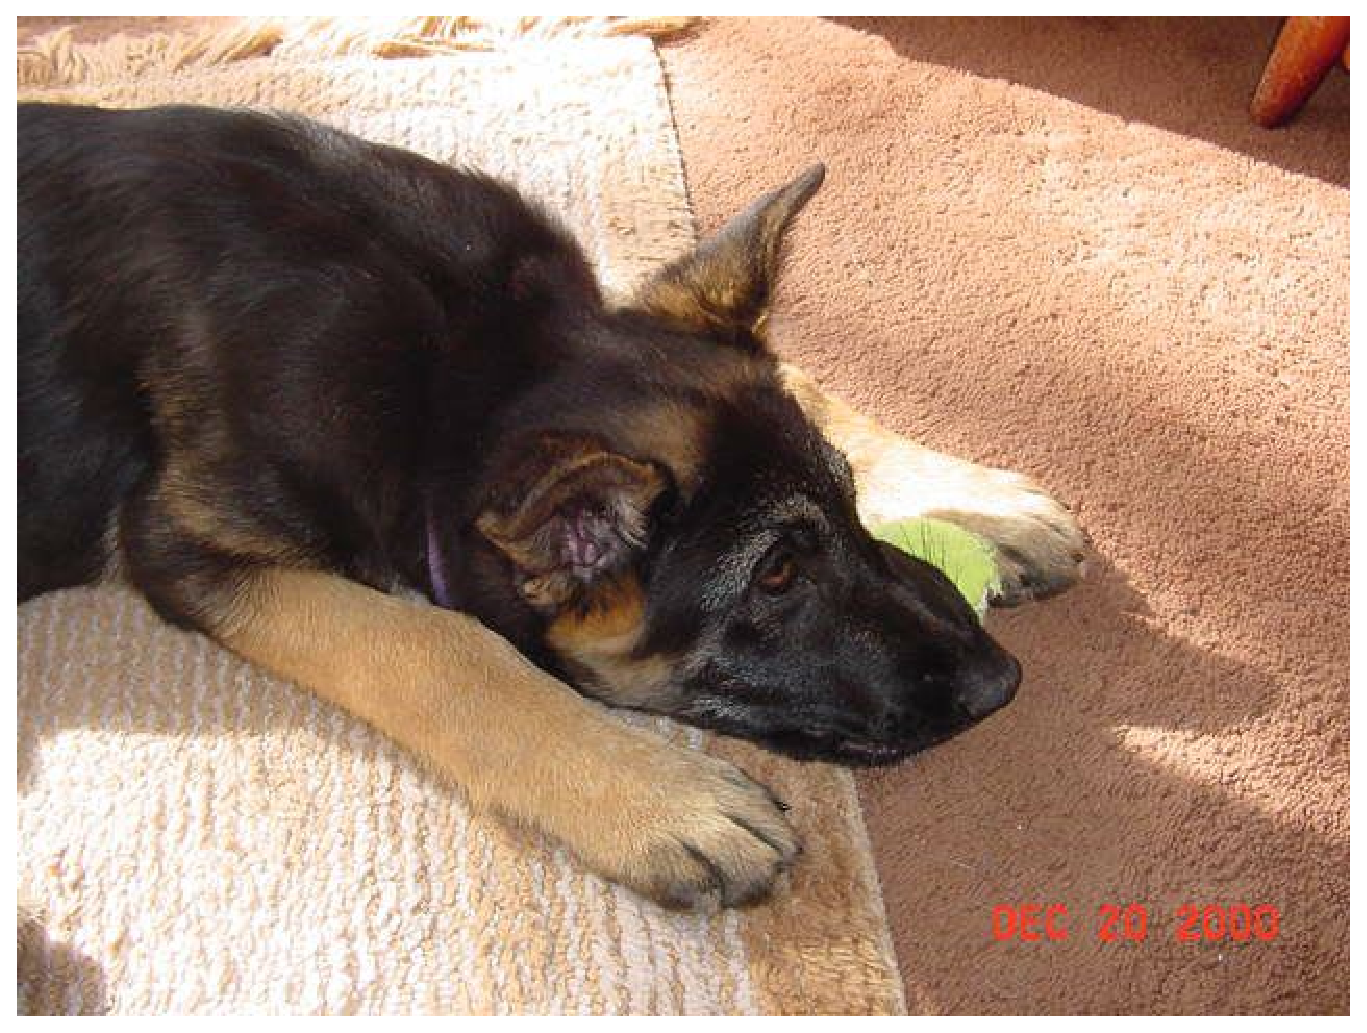
\psfig{file=pup-on-rug.eps,height=1.5in,width=2.0in}
\caption{An example of an imported eps file.}
\label{f:ex}
\end{center}
\end{figure}
\index{commands!environments!figure}%
You can see the commands that generated this
figure in the source file. Look for the line
\cn{begin\{figure\}[htb] \% Imported eps example. }

The command that imports the file is \cn{psfig}, and it also 
controls its size (\texttt{height} and \texttt{width}), and 
can rotate the figure (\texttt{angle}).

Figures can also be drawn by using \LaTeX{} commands. 
Figure \ref{f:circuit} is an example 
(taken from \cite{gms:tlc}).

\begin{figure}[htb] % Picture example.
\begin{center}
   \setlength{\unitlength}{4mm}
   \begin{picture}(12,10)(-2,0)
      \linethickness{0.4pt}
      \qbezier(2.00,6.00)(7.00,6.00)(9.00,3.00)
      \qbezier(2.00,0.00)(7.00,0.00)(9.00,3.00)
      \qbezier(2.00,6.00)(4.00,3.00)(2.00,0.00)
      \qbezier(1.00,6.00)(3.00,3.00)(1.00,0.00)
      \put(9.75,3.00){\circle{1.50}}
      \put(10.50,3.00){\line(1,0){1.50}}
      \put(0.00,5.00){\line(1,0){1.50}}
      \put(0.00,1.00){\line(1,0){1.50}}
   \end{picture}
\caption{An example of a picture}
\label{f:circuit}
\end{center}
\end{figure}
\index{picture}%

The commands that generated this
picture are in the source file following the line
\cn{begin\{figure\}[htb] \% Picture example.  }

The commands used have rather obvious meanings. In particular, 
the command \cn{qbezier} 
\index{commands!qbezier@\cn{qbezier}}%
draws a quadratic Bezier curve, 
defined by its two ending points, and a third point (whose 
coordinates are in the middle) that is used as control point. 
Figure \ref{f:qb} illustrates the effect of the control point:

%\begin{figure}[htb] % Bezier curves example.
\begin{figure}[h] % Bezier curves example.
\begin{center}
   \setlength{\unitlength}{.8mm}
   \begin{picture}(55,55)(-15,0)
      \linethickness{1pt}
      \qbezier(0,0)(-10,30)(50,30)
      \qbezier(0,0)(20,50)(50,30)
      \thinlines
      \put(0,0){\line(-1,3){10}}
      \put(50,30){\line(-1,0){60}}
      \put(0,0){\line(2,5){20}}
      \put(50,30){\line(-3,2){30}}
      \put(0,0){\circle*{1}}
      \put(0,-1){\makebox(0,0)[t]{$A_{0,0}$}}
      \put(-10,30){\circle*{1}}
      \put(-10,31){\makebox(0,0)[b]{$B_{10,30}$}}
      \put(50,30){\circle*{1}}
      \put(58,29){\makebox(0,0)[b]{$C_{50,30}$}}
      \put(20,50){\circle*{1}}
      \put(20,51){\makebox(0,0)[b]{$D_{20,50}$}}
   \end{picture}
\caption{Bezier curves}
\label{f:qb}
\end{center}
\end{figure}
\index{Bezier curves}%


This figure has been generated with the following commands:
\begin{verbatim}
\begin{figure}[htb] % Bezier curves example.
\begin{center}
   \setlength{\unitlength}{.8mm}
   \begin{picture}(55,55)(-15,0)
      \linethickness{1pt}
      \qbezier(0,0)(-10,30)(50,30)
      \qbezier(0,0)(20,50)(50,30)
      \thinlines
      \put(0,0){\line(-1,3){10}}
      \put(50,30){\line(-1,0){60}}
      \put(0,0){\line(2,5){20}}
      \put(50,30){\line(-3,2){30}}
      \put(0,0){\circle*{1}}
      \put(0,-1){\makebox(0,0)[t]{$A_{0,0}$}}
      \put(-10,30){\circle*{1}}
      \put(-10,31){\makebox(0,0)[b]{$B_{10,30}$}}
      \put(50,30){\circle*{1}}
      \put(58,29){\makebox(0,0)[b]{$C_{50,30}$}}
      \put(20,50){\circle*{1}}
      \put(20,51){\makebox(0,0)[b]{$D_{20,50}$}}
   \end{picture}
\caption{Bezier curves}
\label{f:qb}
\end{center}
\end{figure}
\end{verbatim}


\chapter{An Example of Mathematical Writing}
\index{An Example of Mathematical Writing%
@\emph{An Example of Mathematical Writing}}%

\section{Generalized Fatou's Lemma}
\index{Generalized Fatou's Lemma%
@\emph{Generalized Fatou's Lemma}}%

Here we show an application of the following lemma:

\begin{lem}[Generalized Fatou's Lemma] \label{l:fatou}

Let $A$ be a Dedekind ring and $F$ a rational series 
in $A[[X]]$, i.e., $F = p/q$ for some 
$p, q \in A[X]$. Then there exist two polynomials 
$P, Q \in A[X]$ such that $F = P/Q$, 
where $P$ and $Q$ are relatively prime and 
$Q(0) = 1$.

\end{lem}

\proof
See \cite{bertin:psn}, p.~15, theorem~1.3.
\endproof

\begin{thm} \label{l:req}
Let $\{c_n\}_{n=-\infty}^{\infty}$ a set of 
elements from $K$ such that $c_n \in k'$ for every 
$n \geq n_0$, and verifying the following recurrence 
relation of order M:
\begin{equation}
c_n\ =\ r_1\,c_{n-1} + r_2\,c_{n-2} + \dots + r_M\,c_{n-M}
\end{equation}
for every $n \in \mathbb Z$, where $r_1,r_2,\dots,r_M$ are in 
$K$, $r_M \neq 0$. 
Then:

\item{(i)} The coefficients $r_1,r_2,\dots,r_M$ are in 
$k'$, and for every $n \in \mathbb Z$, $c_n \in k'$.

\item{(ii)} If $c_n \in \mathcal O_{k',v}$ 
for every $n \geq n_0$, then the coefficients 
$r_1,r_2,\dots,r_M$ are all in 
$\mathcal O_{k',v}$.

\end{thm}


\proof 

\item{(i)} Let $C_n$ and $R$ be the matrices:

\begin{equation}
C_n\ =
\ \left(
\begin{array}{llll}
              c_n & c_{n+1} & \hdots & c_{n+M-1} \\
              c_{n+1} & c_{n+2} & \hdots  & c_{n+M} \\
              \vdots & \vdots & \ddots & \vdots \\
              c_{n+M-1} & c_{n+M} & \hdots & c_{n+2M-2}
\end{array}
\right)
\end{equation}
and
\begin{equation}
R\ =
\ \left(
\begin{array}{lllll}
              0 & 1 & 0 & \hdots & 0 \\
              0 & 0 & 1 & \hdots & 0 \\
             \vdots & \vdots & \vdots & \ddots & \vdots \\
              0 & 0 & 0 & \hdots & 1 \\
              r_M & r_{M-1} & r_{M-2} & \hdots & r_1 
\end{array}
\right)
\end{equation} 

We have that $C_{n+1} = R\,C_n$. Since the recurrence 
relation is of order M, $C_n$ is non singular. 
On the other hand, $R = C_{n+1}\,C_{n}^{-1}$. Since the 
elements of $C_n$ are in $k'$ for $n \geq n_0$, the entries 
of $R$, and those of $R^{-1}$, will be in $k'$. Since 
$C_{n-1} = R^{-1}\,C_n$, we get that the entries of 
$C_n$ will be in $k'$ also for $n < n_0$. 

\item{(ii)} For each $t \geq n_0$ define the formal 
power series 

\begin{equation}
F_t(X)\ =\ \sum_{n=0}^{\infty} c_{t+n}\,X^n
\end{equation}
which is in $\mathcal O_{k',v}[[X]]$. 
We have $F_t(X) = p_t(X)/q(X)$, 
where $p_t(X),q(X) \in k'[X]$ are the following:
\begin{equation}
p_t(X)\ =\ \sum_{j=0}^{M-1} \Bigl( c_{t+j} - 
                    \sum_{i=1}^{j} r_i\,c_{t+j-i} \Bigr)\,X^j
\end{equation}
\begin{equation}
q(X)\ =\ 1 - r_1\,X - r_2\,X^2 - \dots - r_M\,X^M
\end{equation}
This can be checked by multiplying $F_t(X)$ by $q_t(X)$ 
and using the recurrence relation, which gives 
$F_t(X)\,q(X) = p_t(X)$ (see \cite{poorten:sp}). 

Now we will prove that $p_t(X)$ and $q(X)$ are relatively 
prime. To do so, we will see that they cannot have any 
common root (in $\overline {k'}$). In fact, assume 
that $\alpha$ is a common root of $p_{t_0}(X)$ and $q(X)$ 
for some $t_0 \geq n_0$, i.e.: 
$p_{t_0}(\alpha) = q(\alpha) = 0$. 
Since $q(0)=1$, then $\alpha \neq 0$. Now we have:
\begin{equation}
X\,F_{t_0+1}(X) = F_{t_0}(X) - c_{t_0}
\end{equation}
so:
\begin{multline}
X\,p_{t_0+1}(X) = X\,q(X)\,F_{t_0+1}(X) \\
= q(X)\,(F_{t_0}(X) - c_{t_0}) = p_{t_0}(X) - c_{t_0}\,q(X)
\end{multline}
Hence $p_{t_0+1}(\alpha) = 0$, which means that $\alpha$ is 
also a root of $p_{t_0+1}(X)$. By induction we get that 
$p_t(\alpha) = 0$ for every $t \geq t_0$. Grouping the 
terms of $p_t(X)$ with respect to $c_t,c_{t+1},\dots,c_{t+M-1}$, 
we get:
\begin{equation}
p_t(X) = \sum_{j=0}^{M-1} a_j(X)\,c_{t+j}
\end{equation}
where 
\begin{equation}
a_j(X) = X^j\,\Bigl( 1 - \sum_{i=1}^{M-j-1} r_i\,X^i \Bigr)
\end{equation}
Note that $a_0(X),a_1(X),\dots,a_{M-1}(X)$ do not depend on t. 
On the other hand $p_t(\alpha)=0$ implies
\begin{equation}
\label{e:coldep}
\sum_{j=0}^{M-1} a_j(\alpha)\,c_{t+j} = 0
\end{equation}
for every $t \geq t_0$. Note that $a_{M-1}(\alpha)=\alpha^{M-1}
\neq 0$, so $a_0(\alpha),a_1(\alpha),\dots,a_{M-1}(\alpha)$ 
are not all zero, and (\ref{e:coldep}) means that the columns 
of the matrix $C_{t_0}$ are linearly dependent, so 
$\det C_{t_0}=0$, which contradicts the fact that $C_{t_0}$ 
is non singular. Hence, the hypothesis that $p_t(X)$ and 
$q(X)$ have a common root has to be false. This proves that 
$p_t(X)$ and $q(X)$ are relatively prime. 

By (generalized Fatou's) lemma~\ref{l:fatou}, 
and taking into account that 
$\mathcal O_{k',v}$ is a Dedekind ring, 
we get that there exist two relatively prime 
polynomials $P_t(X)$ and $Q_t(X)$ in 
$\mathcal O_{k',v}[X]$ such that 
$F_t(X) = P_t(X)/Q_t(X)$ and $Q_t(0)=1$. Hence: 
$p_t(X)\,Q_t(X) = q(X)\,P_t(X)$. By unique factorization 
of polynomials in $k'[X]$, there is a $u \in k'$ such that 
$P_t(X) = u\,p_t(X)$ and $Q_t(X) = u\,q_t(X)$. Since 
$Q_t(0)=q(0)=1$, we get that $u=1$, so 
$P_t(X) = p_t(X)$ and $Q_t(X) = q(X)$. 
Hence, the coefficients of $q(X)$ are in 
$\mathcal O_{k',v}$. 

\endproof


\section{Other Examples of Mathematical Writing}

\subsection{An Example of a Commutative Diagram}
\index{An Example of a Commutative Diagram%
@{An Example of a Commutative Diagram}}%

The following is an example of a commutative diagram.
\index{commutative diagram}%
It requires the \texttt{amscd} package.
\index{amscd package@{\texttt{amscd} package}}

\begin{equation*}
\newcommand{\End}{\operatorname{End}}
\begin{CD}
S^{{\mathcal{W}}_\Lambda}\otimes T   @>j>>   T\\
@VVV                                    @VV{\End P}V\\
(S\otimes T)/I                  @=      (Z\otimes T)/J
\end{CD}
\end{equation*}

That diagram has been made with the following commands:

\begin{verbatim}
\newcommand{\End}{\operatorname{End}}
\begin{CD}
S^{{\mathcal{W}}_\Lambda}\otimes T   @>j>>   T\\
@VVV                                    @VV{\End P}V\\
(S\otimes T)/I                  @=      (Z\otimes T)/J
\end{CD}
\end{verbatim}

\subsection{Using AMS Fonts}
\index{Using AMS Fonts@{Using AMS Fonts}}

To use AMS fonts it is necessary to choose from an assortment 
of \LaTeX{} packages. For instance the command 
\cn{usepackage\{amsfonts\}} calls in the \emph{amsfonts} package, 
which provides blackboard bold letters (e.g. $\mathbb{R}$) and 
some math symbols. A superset of that package is 
\emph{amssymb}. Other packages are \emph{eufrak} 
for Frankfurt letters (e.g. $\mathfrak{R}$)
and \emph{eucal} for Euler script 
(e.g. $\mathcal{R}$). 
Consult the \LaTeX{} documentation about this subject 
for additional information.

\appendices
\index{Appendices@\emph{Appendices}}%
\chapter{Lerma's Appendix}
\index{Appendix!Lerma's Appendix@\emph{Lerma's Appendix}}%
The source \LaTeX{} file for this document is no longer quoted in
its entirety in the output document. A \LaTeX{} file can 
include its own source by using the command
\cn{verbatiminput\{\cn{jobname}\}}.


%%%%%%%%%%%%%%%%%%%%%%%%%%%%%%%%%%%%%%%%%%
\chapter{My Appendix \#2}
\index{Appendix!My Appendix \#2@\emph{My Appendix \#2}}%
\section{The First Section}
This is the first section.
This is the second appendix.

\section{The Second Section}
This is the second section of the second appendix.

\subsection{The First Subsection of the Second Section}
This is the first subsection of the second section of the second appendix.

\subsection{The Second Subsection of the Second Section}
This is the second subsection of the second section of the second appendix.

\subsubsection{The First Subsubsection of the Second Subsection of
		the Second Section}
This is the first subsubsection of the second subsection of the
second section of the second appendix.

\subsubsection{The Second Subsubsection of the Second Subsection
		of the Second Section}
This is the second subsubsection of the second subsection of the
second section of the second appendix.

%%%%%%%%%%%%%%%%%%%%%%%%%%%%%%%%%%%%%%%%%%
\chapter{My Appendix \#3}
\index{Appendix!My Appendix \#3@\emph{My Appendix \#3}}%

\section{The First Section}
This is the first section.
This is the third appendix.

\section{The Second Section}
This is the second section of the third appendix.



\end{verbatim}
\index{commands!include@\cn{include}}%
Having the chapters in separate files makes the main .tex file simpler
and allows chapters to be easily re-ordered (just swap the order of the
include commands) or left (commented) out for draft copies.

Note: If you have only one appendix, in addition to using
\cn{appendix} instead of \cn{appendices}, you must leave out the
\cn{chapter} definition at the start of the appendix's text. Putting
it in will cause the insertion of an extra page with only the word
Appendix on it and will cause the appendix to be labeled Appendix 1,
both of which are poor form if there is only one appendix.

If you are writing a short dissertation 
\index{short dissertation}%
that does not require 
chapters, you need to use the command \cn{nochapters} 
\index{commands!nochapters@\cn{nochapters}}%
just before the first section:

\begin{verbatim}
\nochapters 

\section{...}     % First section.
    ... text ... 
\section{...}     % Second section.
    ... text ... 
        (...)
\end{verbatim}

Next comes the bibliography.
\index{bibliography}%
It can be made by hand like this:
\begin{verbatim}
\begin{thebibliography}{foo}
\bibitem ...   
\end{thebibliography}
\end{verbatim}
\index{commands!environments!thebibliography}%
Or it can also be generated with BiB\TeX{}, 
\index{BiBTeX@BiB\TeX{}}%
as explained in chapter \ref{c:bib}.

Finally the vita is produced like this:
\begin{verbatim}
\begin{vita}
     % Insert your brief biographical sketch here. 
     % Your permanent address and the name of the 
     % typist(s) are generated automatically.
\end{vita}

\end{verbatim}

\chapter{Making the Bibliography with BiB\TeX{}}\label{c:bib}
\index{Making the Bibliography with BiBTeX%
@\emph{Making the Bibliography with BiB\TeX{}}}%

BiB\TeX{} 
\index{BiBTeX@BiB\TeX{}}%
allows one to generate automatically the bibliography 
from a database of bibliographic 
items. You need to do the following:

\begin{enumerate}
\item Create the bibliographic database, 
\index{bibliographic database}%
which is a file whose name ends in \texttt{.bib}. 
\index{.bib@\texttt{.bib}}%
Let us call it \texttt{diss.bib}. Entries in this file are like this:
\begin{verbatim}
@BOOK{knuth:tb,
  author = "Donald K. Knuth",
  title = "The \TeXbook",
  publisher = "Addison-Wesley",
  year = "1984",
}
@TECHREPORT{poorten:sp,
  author = "Alf~J.~van der Poorten",
  title = "Some problems of recurrent interest",
  institution = "School of Mathematics and Physics,
                 Macquarie University",
  address = "North Ryde, Australia 2113",
  number = "81-0037",
  month = "August",
  year = "1981",
}
@ARTICLE{erdos:oap,
 author = "Paul Erd{\"o}s and Paul Turan",
 title = "On a problem in the theory of uniform 
          distribution, {I}", 
 journal = "Indag. Math.",
 volume = "10",
 year = "1948",
 pages = "370--378",
}
\end{verbatim}

\item Include a \cn{bibliographystyle} 
\index{commands!bibliographystyle@\cn{bibliographystyle}}%
command in your \LaTeX{} file, say 

\cn{bibliographystyle\{plain\}} 
and a \cn{bibliography} 
\index{commands!bibliography@\cn{bibliography}}%
command to load the bibliography, 
in this case \cn{bibliography\{diss\}}, at the point of your 
document where the bibliography should be inserted. 

The document at this point will look like this:
\begin{verbatim}
\bibliographystyle{plain}
\bibliography{diss}
\end{verbatim}

\item Run \LaTeX{} on your main file, say \texttt{foo.tex}: 
\texttt{latex foo}. This generates an auxiliary file 
\texttt{foo.aux} with a list of \cn{cite} 
\index{commands!cite@\cn{cite}}
references.

\item Run BiB\TeX{} on your file: \texttt{bibtex foo}. 
BiB\TeX{} reads the auxiliary file, looks up the 
bibliographic database (\texttt{diss.bib}), 
and writes a \texttt{.bbl} 
\index{.bbl@\texttt{.bbl}}%
file with the bibliographic information formated according to
the bibliographic style file (\texttt{.bst}, 
\index{.bst@\texttt{.bst}}%
say \texttt{plain.bst}) 
\index{plain.bst@\texttt{plain.bst}}%
specified.  Messages about resources used and error messages
are written to a \texttt{.blg} 
\index{.blg@\texttt{.blg}}%
file (in the case of this template, disstemplate.blg).

\item Run \LaTeX{} again: \texttt{latex foo}, which now 
reads the \texttt{.bbl} 
\index{.bbl@\texttt{.bbl}}%
reference file.

\item Run \LaTeX{} for a third time: \texttt{latex foo}, 
resolving all references.

\end{enumerate}

This includes all bibliographic items that have been cited 
in the document with a \cn{cite} 
\index{commands!cite@\cn{cite}}%
command. In order to include non cited items in the bibliography,
use the command \cn{nocite}. For example, \cn{nocite\{knuth:tb\}}
anywhere in the document (after \cn{begin\{document\}}) includes 
in the bibliography the item with label \texttt{knuth:tb}. 
In order to include \emph{all} items of the bibliographic 
database, use the command \cn{nocite\{*\}}.
\index{commands!nocite@\cn{nocite}}%

\chapter{Making Tables and Including Figures}
\index{Making Tables and Including Figures@\emph{Making Tables
	and Including Figures}}%

The \emph{tabular} 
\index{commands!environments!tabular}%
environment allows us to create complex 
tables and figures, and draw boundaries around and within it.
The following example illustrates this:

\begin{table}[h]
\begin{center}
\caption{An example of a table.}
\vskip 10pt
\begin{tabular}{|ll|l|ll|l|lll|}
\cline{1-2} \cline{4-5} \cline{7-9}
\multicolumn{2}{|c|} {\textsl{Gegenwart}} & &
\multicolumn{2}{|c|} {\textsl{Imperfekt}} & &
\multicolumn{3}{|c|} {\textsl{Perfekt}} \\
\cline{1-2} \cline{4-5} \cline{7-9}
ich & bin  & & ich & war   & & ich & bin  & gewesen \\
du  & bist & & du  & warst & & du  & bist & gewesen \\
er  &      & & er  &       & & er  &      &         \\
sie & ist  & & sie & wart  & & sie & ist  & gewesen \\
es  &      & & es  &       & & es  &      &         \\
\cline{1-2} \cline{4-5} \cline{7-9}
wir & sind & & wir & waren & & wir & sind & gewesen \\
ihr & seid & & ihr & wart  & & ihr & seid & gewesen \\
sie & sind & & sie & waren & & sie & sind & gewesen \\
\cline{1-2} \cline{4-5} \cline{7-9}
Sie & sind & & Sie & waren & & Sie & sind & gewesen \\
\cline{1-2} \cline{4-5} \cline{7-9}
\end{tabular} \\[10pt]
Note: The assistance of Herr Professor Lothar Frommhold \\
in generating this table of German declensions \\
is gratefully acknowledged.
\vskip -20pt
\end{center}
\end{table}
\index{commands!environments!table}%

This table was created with the following sequence 
of commands:
\begin{verbatim}
\begin{table}[h]
\begin{center}
\caption{An example of a table.}
\vskip 10pt
\begin{tabular}{|ll|l|ll|l|lll|}
\cline{1-2} \cline{4-5} \cline{7-9}
\multicolumn{2}{|c|} {\textsl{Gegenwart}} & &
\multicolumn{2}{|c|} {\textsl{Imperfekt}} & &
\multicolumn{3}{|c|} {\textsl{Perfekt}} \\
\cline{1-2} \cline{4-5} \cline{7-9}
ich & bin  & & ich & war   & & ich & bin  & gewesen \\
du  & bist & & du  & warst & & du  & bist & gewesen \\
er  &      & & er  &       & & er  &      &         \\
sie & ist  & & sie & wart  & & sie & ist  & gewesen \\
es  &      & & es  &       & & es  &      &         \\
\cline{1-2} \cline{4-5} \cline{7-9}
wir & sind & & wir & waren & & wir & sind & gewesen \\
ihr & seid & & ihr & wart  & & ihr & seid & gewesen \\
sie & sind & & sie & waren & & sie & sind & gewesen \\
\cline{1-2} \cline{4-5} \cline{7-9}
Sie & sind & & Sie & waren & & Sie & sind & gewesen \\
\cline{1-2} \cline{4-5} \cline{7-9}
\end{tabular} \\[10pt]
Note: The assistance of Herr Professor Lothar Frommhold \\
in generating this table of German declensions \\
is gratefully acknowledged.
\vskip -20pt
\end{center}
\end{table}
\index{commands!environments!table}%
\end{verbatim}

The argument \texttt{h} indicates the position for the 
table, in this case ``here if possible''. Other values
of this argument are:
\texttt{t} (top of the page),
\texttt{b} (bottom of the page),
\texttt{p} (on the page of floats) and 
\texttt{H} (HERE! - requires using the package float.sty.
Note: When this option is used, LaTeX ignores all of its formatting
rules and does what you say, putting the entire float exactly where
it is defined. Check your output to make sure it is what you want!
If you are having trouble with LaTeX wanting to put a figure that's
larger than roughly half-a-page, as well as all of the figures
following it, at the end of a chapter, try using the command
\cn{clearpage} immediately following the large figure --- and maybe
a \cn{newpage} later.)
It is possible to combine several arguments, such as
\texttt{ht} (``here if possible, otherwise on top of
the page''). The default is \texttt{tbp}.

Figure \ref{f:ex} is a typical example of inclusion of a 
figure contained in an encapsulated PostScript file. 
\index{PostScript}%
\index{encapsulated PostScript}%
In order to use it, it is necessary to include the 
command \cn{usepackage\{psfig\}} 
\index{psfig}%
at the beginning of the document.

\begin{figure}[htb] % Imported eps example.
\begin{center}
\ 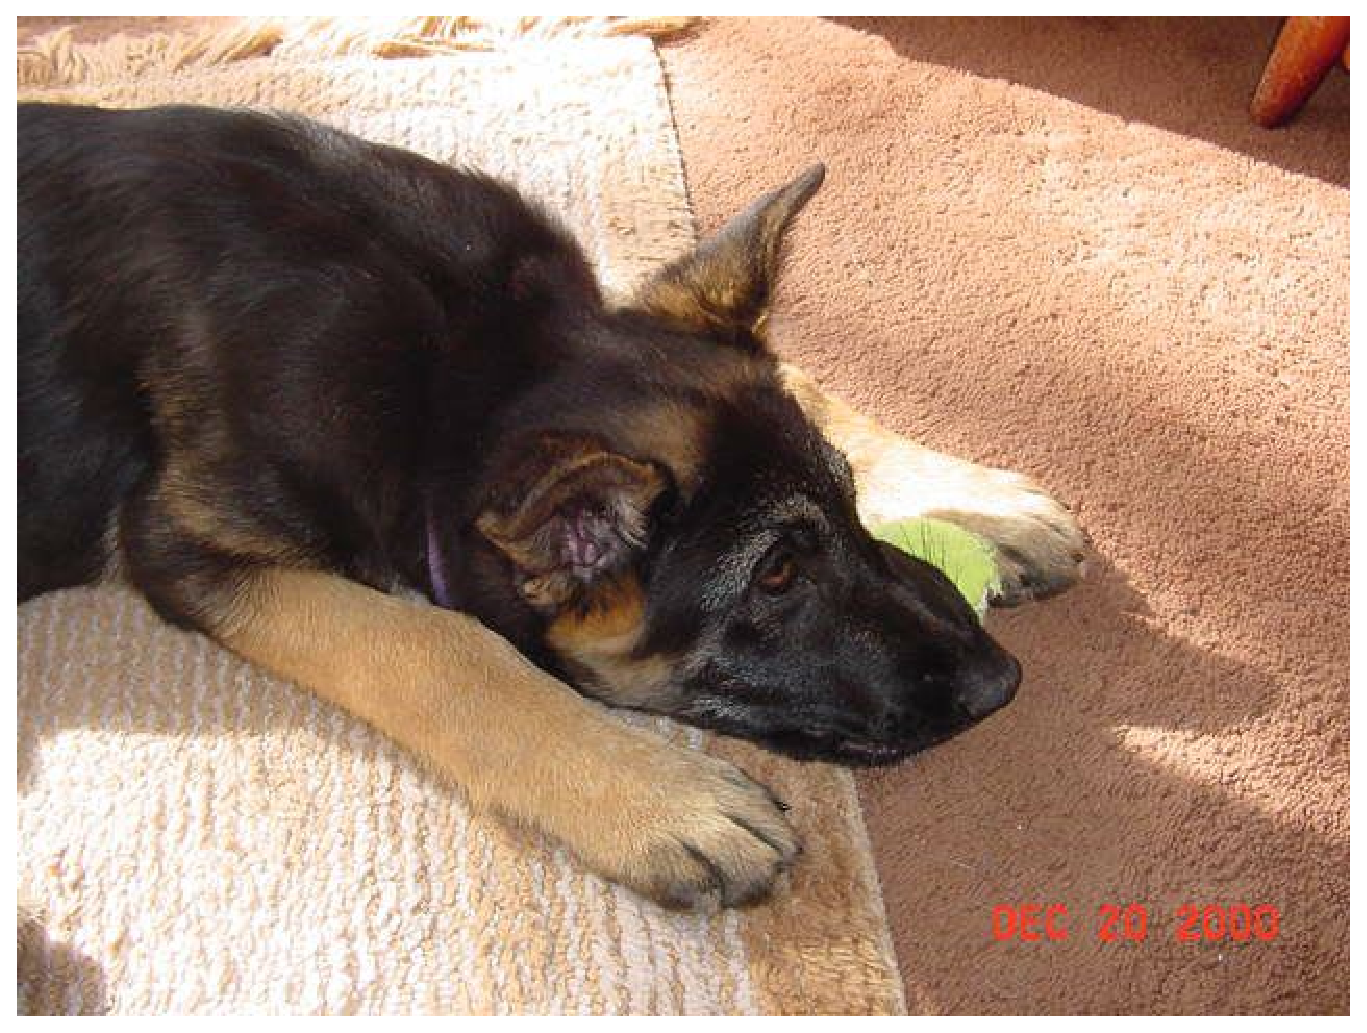
\psfig{file=pup-on-rug.eps,height=1.5in,width=2.0in}
\caption{An example of an imported eps file.}
\label{f:ex}
\end{center}
\end{figure}
\index{commands!environments!figure}%
You can see the commands that generated this
figure in the source file. Look for the line
\cn{begin\{figure\}[htb] \% Imported eps example. }

The command that imports the file is \cn{psfig}, and it also 
controls its size (\texttt{height} and \texttt{width}), and 
can rotate the figure (\texttt{angle}).

Figures can also be drawn by using \LaTeX{} commands. 
Figure \ref{f:circuit} is an example 
(taken from \cite{gms:tlc}).

\begin{figure}[htb] % Picture example.
\begin{center}
   \setlength{\unitlength}{4mm}
   \begin{picture}(12,10)(-2,0)
      \linethickness{0.4pt}
      \qbezier(2.00,6.00)(7.00,6.00)(9.00,3.00)
      \qbezier(2.00,0.00)(7.00,0.00)(9.00,3.00)
      \qbezier(2.00,6.00)(4.00,3.00)(2.00,0.00)
      \qbezier(1.00,6.00)(3.00,3.00)(1.00,0.00)
      \put(9.75,3.00){\circle{1.50}}
      \put(10.50,3.00){\line(1,0){1.50}}
      \put(0.00,5.00){\line(1,0){1.50}}
      \put(0.00,1.00){\line(1,0){1.50}}
   \end{picture}
\caption{An example of a picture}
\label{f:circuit}
\end{center}
\end{figure}
\index{picture}%

The commands that generated this
picture are in the source file following the line
\cn{begin\{figure\}[htb] \% Picture example.  }

The commands used have rather obvious meanings. In particular, 
the command \cn{qbezier} 
\index{commands!qbezier@\cn{qbezier}}%
draws a quadratic Bezier curve, 
defined by its two ending points, and a third point (whose 
coordinates are in the middle) that is used as control point. 
Figure \ref{f:qb} illustrates the effect of the control point:

%\begin{figure}[htb] % Bezier curves example.
\begin{figure}[h] % Bezier curves example.
\begin{center}
   \setlength{\unitlength}{.8mm}
   \begin{picture}(55,55)(-15,0)
      \linethickness{1pt}
      \qbezier(0,0)(-10,30)(50,30)
      \qbezier(0,0)(20,50)(50,30)
      \thinlines
      \put(0,0){\line(-1,3){10}}
      \put(50,30){\line(-1,0){60}}
      \put(0,0){\line(2,5){20}}
      \put(50,30){\line(-3,2){30}}
      \put(0,0){\circle*{1}}
      \put(0,-1){\makebox(0,0)[t]{$A_{0,0}$}}
      \put(-10,30){\circle*{1}}
      \put(-10,31){\makebox(0,0)[b]{$B_{10,30}$}}
      \put(50,30){\circle*{1}}
      \put(58,29){\makebox(0,0)[b]{$C_{50,30}$}}
      \put(20,50){\circle*{1}}
      \put(20,51){\makebox(0,0)[b]{$D_{20,50}$}}
   \end{picture}
\caption{Bezier curves}
\label{f:qb}
\end{center}
\end{figure}
\index{Bezier curves}%


This figure has been generated with the following commands:
\begin{verbatim}
\begin{figure}[htb] % Bezier curves example.
\begin{center}
   \setlength{\unitlength}{.8mm}
   \begin{picture}(55,55)(-15,0)
      \linethickness{1pt}
      \qbezier(0,0)(-10,30)(50,30)
      \qbezier(0,0)(20,50)(50,30)
      \thinlines
      \put(0,0){\line(-1,3){10}}
      \put(50,30){\line(-1,0){60}}
      \put(0,0){\line(2,5){20}}
      \put(50,30){\line(-3,2){30}}
      \put(0,0){\circle*{1}}
      \put(0,-1){\makebox(0,0)[t]{$A_{0,0}$}}
      \put(-10,30){\circle*{1}}
      \put(-10,31){\makebox(0,0)[b]{$B_{10,30}$}}
      \put(50,30){\circle*{1}}
      \put(58,29){\makebox(0,0)[b]{$C_{50,30}$}}
      \put(20,50){\circle*{1}}
      \put(20,51){\makebox(0,0)[b]{$D_{20,50}$}}
   \end{picture}
\caption{Bezier curves}
\label{f:qb}
\end{center}
\end{figure}
\end{verbatim}


\chapter{An Example of Mathematical Writing}
\index{An Example of Mathematical Writing%
@\emph{An Example of Mathematical Writing}}%

\section{Generalized Fatou's Lemma}
\index{Generalized Fatou's Lemma%
@\emph{Generalized Fatou's Lemma}}%

Here we show an application of the following lemma:

\begin{lem}[Generalized Fatou's Lemma] \label{l:fatou}

Let $A$ be a Dedekind ring and $F$ a rational series 
in $A[[X]]$, i.e., $F = p/q$ for some 
$p, q \in A[X]$. Then there exist two polynomials 
$P, Q \in A[X]$ such that $F = P/Q$, 
where $P$ and $Q$ are relatively prime and 
$Q(0) = 1$.

\end{lem}

\proof
See \cite{bertin:psn}, p.~15, theorem~1.3.
\endproof

\begin{thm} \label{l:req}
Let $\{c_n\}_{n=-\infty}^{\infty}$ a set of 
elements from $K$ such that $c_n \in k'$ for every 
$n \geq n_0$, and verifying the following recurrence 
relation of order M:
\begin{equation}
c_n\ =\ r_1\,c_{n-1} + r_2\,c_{n-2} + \dots + r_M\,c_{n-M}
\end{equation}
for every $n \in \mathbb Z$, where $r_1,r_2,\dots,r_M$ are in 
$K$, $r_M \neq 0$. 
Then:

\item{(i)} The coefficients $r_1,r_2,\dots,r_M$ are in 
$k'$, and for every $n \in \mathbb Z$, $c_n \in k'$.

\item{(ii)} If $c_n \in \mathcal O_{k',v}$ 
for every $n \geq n_0$, then the coefficients 
$r_1,r_2,\dots,r_M$ are all in 
$\mathcal O_{k',v}$.

\end{thm}


\proof 

\item{(i)} Let $C_n$ and $R$ be the matrices:

\begin{equation}
C_n\ =
\ \left(
\begin{array}{llll}
              c_n & c_{n+1} & \hdots & c_{n+M-1} \\
              c_{n+1} & c_{n+2} & \hdots  & c_{n+M} \\
              \vdots & \vdots & \ddots & \vdots \\
              c_{n+M-1} & c_{n+M} & \hdots & c_{n+2M-2}
\end{array}
\right)
\end{equation}
and
\begin{equation}
R\ =
\ \left(
\begin{array}{lllll}
              0 & 1 & 0 & \hdots & 0 \\
              0 & 0 & 1 & \hdots & 0 \\
             \vdots & \vdots & \vdots & \ddots & \vdots \\
              0 & 0 & 0 & \hdots & 1 \\
              r_M & r_{M-1} & r_{M-2} & \hdots & r_1 
\end{array}
\right)
\end{equation} 

We have that $C_{n+1} = R\,C_n$. Since the recurrence 
relation is of order M, $C_n$ is non singular. 
On the other hand, $R = C_{n+1}\,C_{n}^{-1}$. Since the 
elements of $C_n$ are in $k'$ for $n \geq n_0$, the entries 
of $R$, and those of $R^{-1}$, will be in $k'$. Since 
$C_{n-1} = R^{-1}\,C_n$, we get that the entries of 
$C_n$ will be in $k'$ also for $n < n_0$. 

\item{(ii)} For each $t \geq n_0$ define the formal 
power series 

\begin{equation}
F_t(X)\ =\ \sum_{n=0}^{\infty} c_{t+n}\,X^n
\end{equation}
which is in $\mathcal O_{k',v}[[X]]$. 
We have $F_t(X) = p_t(X)/q(X)$, 
where $p_t(X),q(X) \in k'[X]$ are the following:
\begin{equation}
p_t(X)\ =\ \sum_{j=0}^{M-1} \Bigl( c_{t+j} - 
                    \sum_{i=1}^{j} r_i\,c_{t+j-i} \Bigr)\,X^j
\end{equation}
\begin{equation}
q(X)\ =\ 1 - r_1\,X - r_2\,X^2 - \dots - r_M\,X^M
\end{equation}
This can be checked by multiplying $F_t(X)$ by $q_t(X)$ 
and using the recurrence relation, which gives 
$F_t(X)\,q(X) = p_t(X)$ (see \cite{poorten:sp}). 

Now we will prove that $p_t(X)$ and $q(X)$ are relatively 
prime. To do so, we will see that they cannot have any 
common root (in $\overline {k'}$). In fact, assume 
that $\alpha$ is a common root of $p_{t_0}(X)$ and $q(X)$ 
for some $t_0 \geq n_0$, i.e.: 
$p_{t_0}(\alpha) = q(\alpha) = 0$. 
Since $q(0)=1$, then $\alpha \neq 0$. Now we have:
\begin{equation}
X\,F_{t_0+1}(X) = F_{t_0}(X) - c_{t_0}
\end{equation}
so:
\begin{multline}
X\,p_{t_0+1}(X) = X\,q(X)\,F_{t_0+1}(X) \\
= q(X)\,(F_{t_0}(X) - c_{t_0}) = p_{t_0}(X) - c_{t_0}\,q(X)
\end{multline}
Hence $p_{t_0+1}(\alpha) = 0$, which means that $\alpha$ is 
also a root of $p_{t_0+1}(X)$. By induction we get that 
$p_t(\alpha) = 0$ for every $t \geq t_0$. Grouping the 
terms of $p_t(X)$ with respect to $c_t,c_{t+1},\dots,c_{t+M-1}$, 
we get:
\begin{equation}
p_t(X) = \sum_{j=0}^{M-1} a_j(X)\,c_{t+j}
\end{equation}
where 
\begin{equation}
a_j(X) = X^j\,\Bigl( 1 - \sum_{i=1}^{M-j-1} r_i\,X^i \Bigr)
\end{equation}
Note that $a_0(X),a_1(X),\dots,a_{M-1}(X)$ do not depend on t. 
On the other hand $p_t(\alpha)=0$ implies
\begin{equation}
\label{e:coldep}
\sum_{j=0}^{M-1} a_j(\alpha)\,c_{t+j} = 0
\end{equation}
for every $t \geq t_0$. Note that $a_{M-1}(\alpha)=\alpha^{M-1}
\neq 0$, so $a_0(\alpha),a_1(\alpha),\dots,a_{M-1}(\alpha)$ 
are not all zero, and (\ref{e:coldep}) means that the columns 
of the matrix $C_{t_0}$ are linearly dependent, so 
$\det C_{t_0}=0$, which contradicts the fact that $C_{t_0}$ 
is non singular. Hence, the hypothesis that $p_t(X)$ and 
$q(X)$ have a common root has to be false. This proves that 
$p_t(X)$ and $q(X)$ are relatively prime. 

By (generalized Fatou's) lemma~\ref{l:fatou}, 
and taking into account that 
$\mathcal O_{k',v}$ is a Dedekind ring, 
we get that there exist two relatively prime 
polynomials $P_t(X)$ and $Q_t(X)$ in 
$\mathcal O_{k',v}[X]$ such that 
$F_t(X) = P_t(X)/Q_t(X)$ and $Q_t(0)=1$. Hence: 
$p_t(X)\,Q_t(X) = q(X)\,P_t(X)$. By unique factorization 
of polynomials in $k'[X]$, there is a $u \in k'$ such that 
$P_t(X) = u\,p_t(X)$ and $Q_t(X) = u\,q_t(X)$. Since 
$Q_t(0)=q(0)=1$, we get that $u=1$, so 
$P_t(X) = p_t(X)$ and $Q_t(X) = q(X)$. 
Hence, the coefficients of $q(X)$ are in 
$\mathcal O_{k',v}$. 

\endproof


\section{Other Examples of Mathematical Writing}

\subsection{An Example of a Commutative Diagram}
\index{An Example of a Commutative Diagram%
@{An Example of a Commutative Diagram}}%

The following is an example of a commutative diagram.
\index{commutative diagram}%
It requires the \texttt{amscd} package.
\index{amscd package@{\texttt{amscd} package}}

\begin{equation*}
\newcommand{\End}{\operatorname{End}}
\begin{CD}
S^{{\mathcal{W}}_\Lambda}\otimes T   @>j>>   T\\
@VVV                                    @VV{\End P}V\\
(S\otimes T)/I                  @=      (Z\otimes T)/J
\end{CD}
\end{equation*}

That diagram has been made with the following commands:

\begin{verbatim}
\newcommand{\End}{\operatorname{End}}
\begin{CD}
S^{{\mathcal{W}}_\Lambda}\otimes T   @>j>>   T\\
@VVV                                    @VV{\End P}V\\
(S\otimes T)/I                  @=      (Z\otimes T)/J
\end{CD}
\end{verbatim}

\subsection{Using AMS Fonts}
\index{Using AMS Fonts@{Using AMS Fonts}}

To use AMS fonts it is necessary to choose from an assortment 
of \LaTeX{} packages. For instance the command 
\cn{usepackage\{amsfonts\}} calls in the \emph{amsfonts} package, 
which provides blackboard bold letters (e.g. $\mathbb{R}$) and 
some math symbols. A superset of that package is 
\emph{amssymb}. Other packages are \emph{eufrak} 
for Frankfurt letters (e.g. $\mathfrak{R}$)
and \emph{eucal} for Euler script 
(e.g. $\mathcal{R}$). 
Consult the \LaTeX{} documentation about this subject 
for additional information.

\appendices
\index{Appendices@\emph{Appendices}}%
\chapter{Lerma's Appendix}
\index{Appendix!Lerma's Appendix@\emph{Lerma's Appendix}}%
The source \LaTeX{} file for this document is no longer quoted in
its entirety in the output document. A \LaTeX{} file can 
include its own source by using the command
\cn{verbatiminput\{\cn{jobname}\}}.


%%%%%%%%%%%%%%%%%%%%%%%%%%%%%%%%%%%%%%%%%%
\chapter{My Appendix \#2}
\index{Appendix!My Appendix \#2@\emph{My Appendix \#2}}%
\section{The First Section}
This is the first section.
This is the second appendix.

\section{The Second Section}
This is the second section of the second appendix.

\subsection{The First Subsection of the Second Section}
This is the first subsection of the second section of the second appendix.

\subsection{The Second Subsection of the Second Section}
This is the second subsection of the second section of the second appendix.

\subsubsection{The First Subsubsection of the Second Subsection of
		the Second Section}
This is the first subsubsection of the second subsection of the
second section of the second appendix.

\subsubsection{The Second Subsubsection of the Second Subsection
		of the Second Section}
This is the second subsubsection of the second subsection of the
second section of the second appendix.

%%%%%%%%%%%%%%%%%%%%%%%%%%%%%%%%%%%%%%%%%%
\chapter{My Appendix \#3}
\index{Appendix!My Appendix \#3@\emph{My Appendix \#3}}%

\section{The First Section}
This is the first section.
This is the third appendix.

\section{The Second Section}
This is the second section of the third appendix.



\end{verbatim}
\index{commands!include@\cn{include}}%
Having the chapters in separate files makes the main .tex file simpler
and allows chapters to be easily re-ordered (just swap the order of the
include commands) or left (commented) out for draft copies.

Note: If you have only one appendix, in addition to using
\cn{appendix} instead of \cn{appendices}, you must leave out the
\cn{chapter} definition at the start of the appendix's text. Putting
it in will cause the insertion of an extra page with only the word
Appendix on it and will cause the appendix to be labeled Appendix 1,
both of which are poor form if there is only one appendix.

If you are writing a short dissertation 
\index{short dissertation}%
that does not require 
chapters, you need to use the command \cn{nochapters} 
\index{commands!nochapters@\cn{nochapters}}%
just before the first section:

\begin{verbatim}
\nochapters 

\section{...}     % First section.
    ... text ... 
\section{...}     % Second section.
    ... text ... 
        (...)
\end{verbatim}

Next comes the bibliography.
\index{bibliography}%
It can be made by hand like this:
\begin{verbatim}
\begin{thebibliography}{foo}
\bibitem ...   
\end{thebibliography}
\end{verbatim}
\index{commands!environments!thebibliography}%
Or it can also be generated with BiB\TeX{}, 
\index{BiBTeX@BiB\TeX{}}%
as explained in chapter \ref{c:bib}.

Finally the vita is produced like this:
\begin{verbatim}
\begin{vita}
     % Insert your brief biographical sketch here. 
     % Your permanent address and the name of the 
     % typist(s) are generated automatically.
\end{vita}

\end{verbatim}

\chapter{Making the Bibliography with BiB\TeX{}}\label{c:bib}
\index{Making the Bibliography with BiBTeX%
@\emph{Making the Bibliography with BiB\TeX{}}}%

BiB\TeX{} 
\index{BiBTeX@BiB\TeX{}}%
allows one to generate automatically the bibliography 
from a database of bibliographic 
items. You need to do the following:

\begin{enumerate}
\item Create the bibliographic database, 
\index{bibliographic database}%
which is a file whose name ends in \texttt{.bib}. 
\index{.bib@\texttt{.bib}}%
Let us call it \texttt{diss.bib}. Entries in this file are like this:
\begin{verbatim}
@BOOK{knuth:tb,
  author = "Donald K. Knuth",
  title = "The \TeXbook",
  publisher = "Addison-Wesley",
  year = "1984",
}
@TECHREPORT{poorten:sp,
  author = "Alf~J.~van der Poorten",
  title = "Some problems of recurrent interest",
  institution = "School of Mathematics and Physics,
                 Macquarie University",
  address = "North Ryde, Australia 2113",
  number = "81-0037",
  month = "August",
  year = "1981",
}
@ARTICLE{erdos:oap,
 author = "Paul Erd{\"o}s and Paul Turan",
 title = "On a problem in the theory of uniform 
          distribution, {I}", 
 journal = "Indag. Math.",
 volume = "10",
 year = "1948",
 pages = "370--378",
}
\end{verbatim}

\item Include a \cn{bibliographystyle} 
\index{commands!bibliographystyle@\cn{bibliographystyle}}%
command in your \LaTeX{} file, say 

\cn{bibliographystyle\{plain\}} 
and a \cn{bibliography} 
\index{commands!bibliography@\cn{bibliography}}%
command to load the bibliography, 
in this case \cn{bibliography\{diss\}}, at the point of your 
document where the bibliography should be inserted. 

The document at this point will look like this:
\begin{verbatim}
\bibliographystyle{plain}
\bibliography{diss}
\end{verbatim}

\item Run \LaTeX{} on your main file, say \texttt{foo.tex}: 
\texttt{latex foo}. This generates an auxiliary file 
\texttt{foo.aux} with a list of \cn{cite} 
\index{commands!cite@\cn{cite}}
references.

\item Run BiB\TeX{} on your file: \texttt{bibtex foo}. 
BiB\TeX{} reads the auxiliary file, looks up the 
bibliographic database (\texttt{diss.bib}), 
and writes a \texttt{.bbl} 
\index{.bbl@\texttt{.bbl}}%
file with the bibliographic information formated according to
the bibliographic style file (\texttt{.bst}, 
\index{.bst@\texttt{.bst}}%
say \texttt{plain.bst}) 
\index{plain.bst@\texttt{plain.bst}}%
specified.  Messages about resources used and error messages
are written to a \texttt{.blg} 
\index{.blg@\texttt{.blg}}%
file (in the case of this template, disstemplate.blg).

\item Run \LaTeX{} again: \texttt{latex foo}, which now 
reads the \texttt{.bbl} 
\index{.bbl@\texttt{.bbl}}%
reference file.

\item Run \LaTeX{} for a third time: \texttt{latex foo}, 
resolving all references.

\end{enumerate}

This includes all bibliographic items that have been cited 
in the document with a \cn{cite} 
\index{commands!cite@\cn{cite}}%
command. In order to include non cited items in the bibliography,
use the command \cn{nocite}. For example, \cn{nocite\{knuth:tb\}}
anywhere in the document (after \cn{begin\{document\}}) includes 
in the bibliography the item with label \texttt{knuth:tb}. 
In order to include \emph{all} items of the bibliographic 
database, use the command \cn{nocite\{*\}}.
\index{commands!nocite@\cn{nocite}}%

\chapter{Making Tables and Including Figures}
\index{Making Tables and Including Figures@\emph{Making Tables
	and Including Figures}}%

The \emph{tabular} 
\index{commands!environments!tabular}%
environment allows us to create complex 
tables and figures, and draw boundaries around and within it.
The following example illustrates this:

\begin{table}[h]
\begin{center}
\caption{An example of a table.}
\vskip 10pt
\begin{tabular}{|ll|l|ll|l|lll|}
\cline{1-2} \cline{4-5} \cline{7-9}
\multicolumn{2}{|c|} {\textsl{Gegenwart}} & &
\multicolumn{2}{|c|} {\textsl{Imperfekt}} & &
\multicolumn{3}{|c|} {\textsl{Perfekt}} \\
\cline{1-2} \cline{4-5} \cline{7-9}
ich & bin  & & ich & war   & & ich & bin  & gewesen \\
du  & bist & & du  & warst & & du  & bist & gewesen \\
er  &      & & er  &       & & er  &      &         \\
sie & ist  & & sie & wart  & & sie & ist  & gewesen \\
es  &      & & es  &       & & es  &      &         \\
\cline{1-2} \cline{4-5} \cline{7-9}
wir & sind & & wir & waren & & wir & sind & gewesen \\
ihr & seid & & ihr & wart  & & ihr & seid & gewesen \\
sie & sind & & sie & waren & & sie & sind & gewesen \\
\cline{1-2} \cline{4-5} \cline{7-9}
Sie & sind & & Sie & waren & & Sie & sind & gewesen \\
\cline{1-2} \cline{4-5} \cline{7-9}
\end{tabular} \\[10pt]
Note: The assistance of Herr Professor Lothar Frommhold \\
in generating this table of German declensions \\
is gratefully acknowledged.
\vskip -20pt
\end{center}
\end{table}
\index{commands!environments!table}%

This table was created with the following sequence 
of commands:
\begin{verbatim}
\begin{table}[h]
\begin{center}
\caption{An example of a table.}
\vskip 10pt
\begin{tabular}{|ll|l|ll|l|lll|}
\cline{1-2} \cline{4-5} \cline{7-9}
\multicolumn{2}{|c|} {\textsl{Gegenwart}} & &
\multicolumn{2}{|c|} {\textsl{Imperfekt}} & &
\multicolumn{3}{|c|} {\textsl{Perfekt}} \\
\cline{1-2} \cline{4-5} \cline{7-9}
ich & bin  & & ich & war   & & ich & bin  & gewesen \\
du  & bist & & du  & warst & & du  & bist & gewesen \\
er  &      & & er  &       & & er  &      &         \\
sie & ist  & & sie & wart  & & sie & ist  & gewesen \\
es  &      & & es  &       & & es  &      &         \\
\cline{1-2} \cline{4-5} \cline{7-9}
wir & sind & & wir & waren & & wir & sind & gewesen \\
ihr & seid & & ihr & wart  & & ihr & seid & gewesen \\
sie & sind & & sie & waren & & sie & sind & gewesen \\
\cline{1-2} \cline{4-5} \cline{7-9}
Sie & sind & & Sie & waren & & Sie & sind & gewesen \\
\cline{1-2} \cline{4-5} \cline{7-9}
\end{tabular} \\[10pt]
Note: The assistance of Herr Professor Lothar Frommhold \\
in generating this table of German declensions \\
is gratefully acknowledged.
\vskip -20pt
\end{center}
\end{table}
\index{commands!environments!table}%
\end{verbatim}

The argument \texttt{h} indicates the position for the 
table, in this case ``here if possible''. Other values
of this argument are:
\texttt{t} (top of the page),
\texttt{b} (bottom of the page),
\texttt{p} (on the page of floats) and 
\texttt{H} (HERE! - requires using the package float.sty.
Note: When this option is used, LaTeX ignores all of its formatting
rules and does what you say, putting the entire float exactly where
it is defined. Check your output to make sure it is what you want!
If you are having trouble with LaTeX wanting to put a figure that's
larger than roughly half-a-page, as well as all of the figures
following it, at the end of a chapter, try using the command
\cn{clearpage} immediately following the large figure --- and maybe
a \cn{newpage} later.)
It is possible to combine several arguments, such as
\texttt{ht} (``here if possible, otherwise on top of
the page''). The default is \texttt{tbp}.

Figure \ref{f:ex} is a typical example of inclusion of a 
figure contained in an encapsulated PostScript file. 
\index{PostScript}%
\index{encapsulated PostScript}%
In order to use it, it is necessary to include the 
command \cn{usepackage\{psfig\}} 
\index{psfig}%
at the beginning of the document.

\begin{figure}[htb] % Imported eps example.
\begin{center}
\ 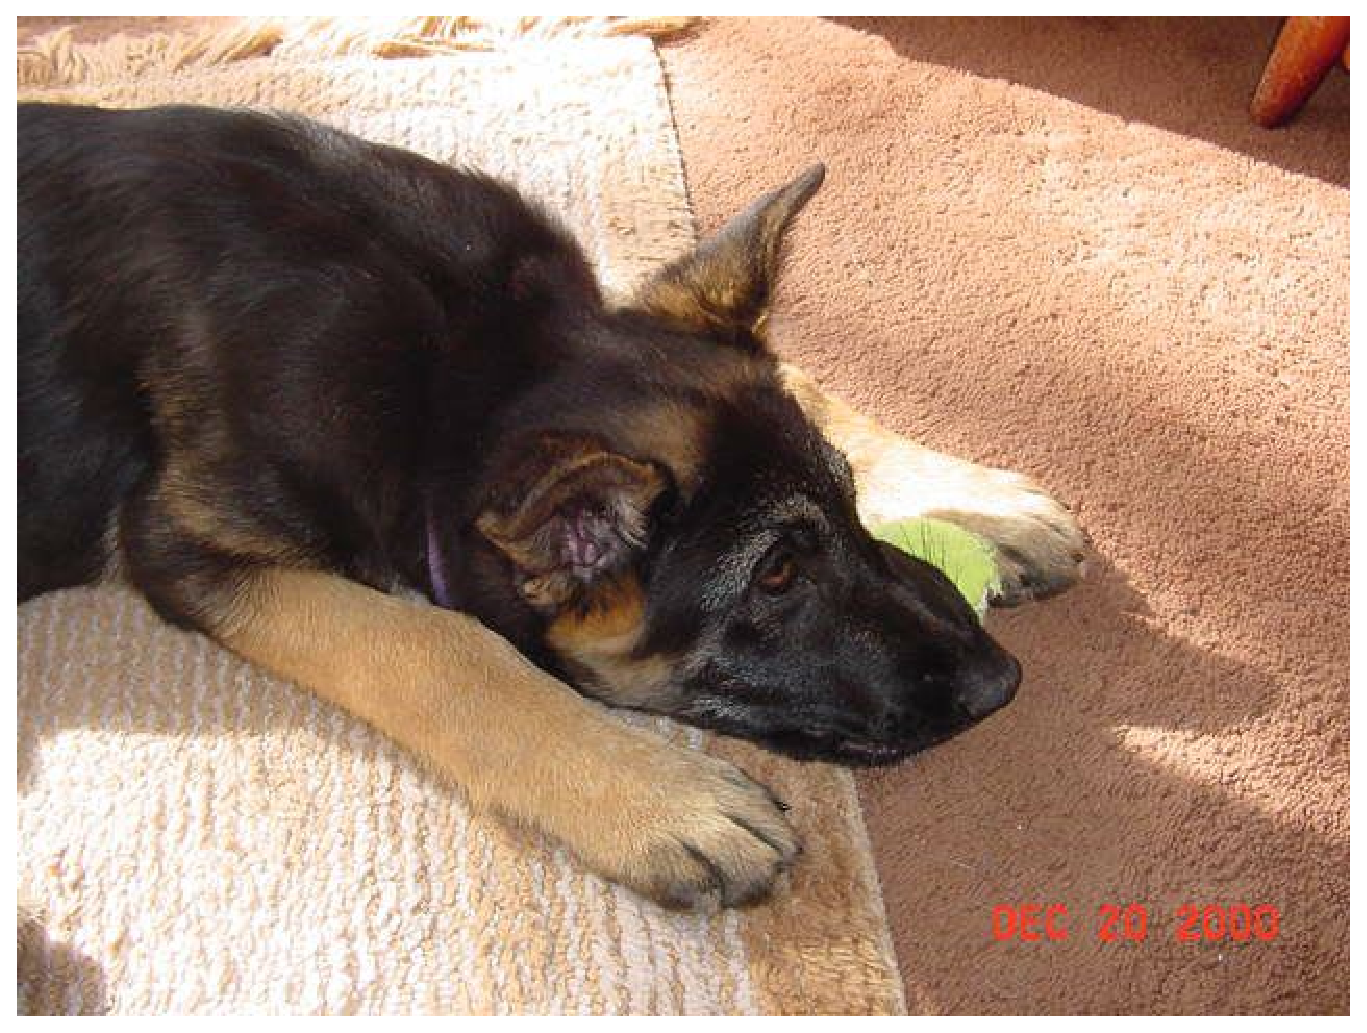
\psfig{file=pup-on-rug.eps,height=1.5in,width=2.0in}
\caption{An example of an imported eps file.}
\label{f:ex}
\end{center}
\end{figure}
\index{commands!environments!figure}%
You can see the commands that generated this
figure in the source file. Look for the line
\cn{begin\{figure\}[htb] \% Imported eps example. }

The command that imports the file is \cn{psfig}, and it also 
controls its size (\texttt{height} and \texttt{width}), and 
can rotate the figure (\texttt{angle}).

Figures can also be drawn by using \LaTeX{} commands. 
Figure \ref{f:circuit} is an example 
(taken from \cite{gms:tlc}).

\begin{figure}[htb] % Picture example.
\begin{center}
   \setlength{\unitlength}{4mm}
   \begin{picture}(12,10)(-2,0)
      \linethickness{0.4pt}
      \qbezier(2.00,6.00)(7.00,6.00)(9.00,3.00)
      \qbezier(2.00,0.00)(7.00,0.00)(9.00,3.00)
      \qbezier(2.00,6.00)(4.00,3.00)(2.00,0.00)
      \qbezier(1.00,6.00)(3.00,3.00)(1.00,0.00)
      \put(9.75,3.00){\circle{1.50}}
      \put(10.50,3.00){\line(1,0){1.50}}
      \put(0.00,5.00){\line(1,0){1.50}}
      \put(0.00,1.00){\line(1,0){1.50}}
   \end{picture}
\caption{An example of a picture}
\label{f:circuit}
\end{center}
\end{figure}
\index{picture}%

The commands that generated this
picture are in the source file following the line
\cn{begin\{figure\}[htb] \% Picture example.  }

The commands used have rather obvious meanings. In particular, 
the command \cn{qbezier} 
\index{commands!qbezier@\cn{qbezier}}%
draws a quadratic Bezier curve, 
defined by its two ending points, and a third point (whose 
coordinates are in the middle) that is used as control point. 
Figure \ref{f:qb} illustrates the effect of the control point:

%\begin{figure}[htb] % Bezier curves example.
\begin{figure}[h] % Bezier curves example.
\begin{center}
   \setlength{\unitlength}{.8mm}
   \begin{picture}(55,55)(-15,0)
      \linethickness{1pt}
      \qbezier(0,0)(-10,30)(50,30)
      \qbezier(0,0)(20,50)(50,30)
      \thinlines
      \put(0,0){\line(-1,3){10}}
      \put(50,30){\line(-1,0){60}}
      \put(0,0){\line(2,5){20}}
      \put(50,30){\line(-3,2){30}}
      \put(0,0){\circle*{1}}
      \put(0,-1){\makebox(0,0)[t]{$A_{0,0}$}}
      \put(-10,30){\circle*{1}}
      \put(-10,31){\makebox(0,0)[b]{$B_{10,30}$}}
      \put(50,30){\circle*{1}}
      \put(58,29){\makebox(0,0)[b]{$C_{50,30}$}}
      \put(20,50){\circle*{1}}
      \put(20,51){\makebox(0,0)[b]{$D_{20,50}$}}
   \end{picture}
\caption{Bezier curves}
\label{f:qb}
\end{center}
\end{figure}
\index{Bezier curves}%


This figure has been generated with the following commands:
\begin{verbatim}
\begin{figure}[htb] % Bezier curves example.
\begin{center}
   \setlength{\unitlength}{.8mm}
   \begin{picture}(55,55)(-15,0)
      \linethickness{1pt}
      \qbezier(0,0)(-10,30)(50,30)
      \qbezier(0,0)(20,50)(50,30)
      \thinlines
      \put(0,0){\line(-1,3){10}}
      \put(50,30){\line(-1,0){60}}
      \put(0,0){\line(2,5){20}}
      \put(50,30){\line(-3,2){30}}
      \put(0,0){\circle*{1}}
      \put(0,-1){\makebox(0,0)[t]{$A_{0,0}$}}
      \put(-10,30){\circle*{1}}
      \put(-10,31){\makebox(0,0)[b]{$B_{10,30}$}}
      \put(50,30){\circle*{1}}
      \put(58,29){\makebox(0,0)[b]{$C_{50,30}$}}
      \put(20,50){\circle*{1}}
      \put(20,51){\makebox(0,0)[b]{$D_{20,50}$}}
   \end{picture}
\caption{Bezier curves}
\label{f:qb}
\end{center}
\end{figure}
\end{verbatim}


\chapter{An Example of Mathematical Writing}
\index{An Example of Mathematical Writing%
@\emph{An Example of Mathematical Writing}}%

\section{Generalized Fatou's Lemma}
\index{Generalized Fatou's Lemma%
@\emph{Generalized Fatou's Lemma}}%

Here we show an application of the following lemma:

\begin{lem}[Generalized Fatou's Lemma] \label{l:fatou}

Let $A$ be a Dedekind ring and $F$ a rational series 
in $A[[X]]$, i.e., $F = p/q$ for some 
$p, q \in A[X]$. Then there exist two polynomials 
$P, Q \in A[X]$ such that $F = P/Q$, 
where $P$ and $Q$ are relatively prime and 
$Q(0) = 1$.

\end{lem}

\proof
See \cite{bertin:psn}, p.~15, theorem~1.3.
\endproof

\begin{thm} \label{l:req}
Let $\{c_n\}_{n=-\infty}^{\infty}$ a set of 
elements from $K$ such that $c_n \in k'$ for every 
$n \geq n_0$, and verifying the following recurrence 
relation of order M:
\begin{equation}
c_n\ =\ r_1\,c_{n-1} + r_2\,c_{n-2} + \dots + r_M\,c_{n-M}
\end{equation}
for every $n \in \mathbb Z$, where $r_1,r_2,\dots,r_M$ are in 
$K$, $r_M \neq 0$. 
Then:

\item{(i)} The coefficients $r_1,r_2,\dots,r_M$ are in 
$k'$, and for every $n \in \mathbb Z$, $c_n \in k'$.

\item{(ii)} If $c_n \in \mathcal O_{k',v}$ 
for every $n \geq n_0$, then the coefficients 
$r_1,r_2,\dots,r_M$ are all in 
$\mathcal O_{k',v}$.

\end{thm}


\proof 

\item{(i)} Let $C_n$ and $R$ be the matrices:

\begin{equation}
C_n\ =
\ \left(
\begin{array}{llll}
              c_n & c_{n+1} & \hdots & c_{n+M-1} \\
              c_{n+1} & c_{n+2} & \hdots  & c_{n+M} \\
              \vdots & \vdots & \ddots & \vdots \\
              c_{n+M-1} & c_{n+M} & \hdots & c_{n+2M-2}
\end{array}
\right)
\end{equation}
and
\begin{equation}
R\ =
\ \left(
\begin{array}{lllll}
              0 & 1 & 0 & \hdots & 0 \\
              0 & 0 & 1 & \hdots & 0 \\
             \vdots & \vdots & \vdots & \ddots & \vdots \\
              0 & 0 & 0 & \hdots & 1 \\
              r_M & r_{M-1} & r_{M-2} & \hdots & r_1 
\end{array}
\right)
\end{equation} 

We have that $C_{n+1} = R\,C_n$. Since the recurrence 
relation is of order M, $C_n$ is non singular. 
On the other hand, $R = C_{n+1}\,C_{n}^{-1}$. Since the 
elements of $C_n$ are in $k'$ for $n \geq n_0$, the entries 
of $R$, and those of $R^{-1}$, will be in $k'$. Since 
$C_{n-1} = R^{-1}\,C_n$, we get that the entries of 
$C_n$ will be in $k'$ also for $n < n_0$. 

\item{(ii)} For each $t \geq n_0$ define the formal 
power series 

\begin{equation}
F_t(X)\ =\ \sum_{n=0}^{\infty} c_{t+n}\,X^n
\end{equation}
which is in $\mathcal O_{k',v}[[X]]$. 
We have $F_t(X) = p_t(X)/q(X)$, 
where $p_t(X),q(X) \in k'[X]$ are the following:
\begin{equation}
p_t(X)\ =\ \sum_{j=0}^{M-1} \Bigl( c_{t+j} - 
                    \sum_{i=1}^{j} r_i\,c_{t+j-i} \Bigr)\,X^j
\end{equation}
\begin{equation}
q(X)\ =\ 1 - r_1\,X - r_2\,X^2 - \dots - r_M\,X^M
\end{equation}
This can be checked by multiplying $F_t(X)$ by $q_t(X)$ 
and using the recurrence relation, which gives 
$F_t(X)\,q(X) = p_t(X)$ (see \cite{poorten:sp}). 

Now we will prove that $p_t(X)$ and $q(X)$ are relatively 
prime. To do so, we will see that they cannot have any 
common root (in $\overline {k'}$). In fact, assume 
that $\alpha$ is a common root of $p_{t_0}(X)$ and $q(X)$ 
for some $t_0 \geq n_0$, i.e.: 
$p_{t_0}(\alpha) = q(\alpha) = 0$. 
Since $q(0)=1$, then $\alpha \neq 0$. Now we have:
\begin{equation}
X\,F_{t_0+1}(X) = F_{t_0}(X) - c_{t_0}
\end{equation}
so:
\begin{multline}
X\,p_{t_0+1}(X) = X\,q(X)\,F_{t_0+1}(X) \\
= q(X)\,(F_{t_0}(X) - c_{t_0}) = p_{t_0}(X) - c_{t_0}\,q(X)
\end{multline}
Hence $p_{t_0+1}(\alpha) = 0$, which means that $\alpha$ is 
also a root of $p_{t_0+1}(X)$. By induction we get that 
$p_t(\alpha) = 0$ for every $t \geq t_0$. Grouping the 
terms of $p_t(X)$ with respect to $c_t,c_{t+1},\dots,c_{t+M-1}$, 
we get:
\begin{equation}
p_t(X) = \sum_{j=0}^{M-1} a_j(X)\,c_{t+j}
\end{equation}
where 
\begin{equation}
a_j(X) = X^j\,\Bigl( 1 - \sum_{i=1}^{M-j-1} r_i\,X^i \Bigr)
\end{equation}
Note that $a_0(X),a_1(X),\dots,a_{M-1}(X)$ do not depend on t. 
On the other hand $p_t(\alpha)=0$ implies
\begin{equation}
\label{e:coldep}
\sum_{j=0}^{M-1} a_j(\alpha)\,c_{t+j} = 0
\end{equation}
for every $t \geq t_0$. Note that $a_{M-1}(\alpha)=\alpha^{M-1}
\neq 0$, so $a_0(\alpha),a_1(\alpha),\dots,a_{M-1}(\alpha)$ 
are not all zero, and (\ref{e:coldep}) means that the columns 
of the matrix $C_{t_0}$ are linearly dependent, so 
$\det C_{t_0}=0$, which contradicts the fact that $C_{t_0}$ 
is non singular. Hence, the hypothesis that $p_t(X)$ and 
$q(X)$ have a common root has to be false. This proves that 
$p_t(X)$ and $q(X)$ are relatively prime. 

By (generalized Fatou's) lemma~\ref{l:fatou}, 
and taking into account that 
$\mathcal O_{k',v}$ is a Dedekind ring, 
we get that there exist two relatively prime 
polynomials $P_t(X)$ and $Q_t(X)$ in 
$\mathcal O_{k',v}[X]$ such that 
$F_t(X) = P_t(X)/Q_t(X)$ and $Q_t(0)=1$. Hence: 
$p_t(X)\,Q_t(X) = q(X)\,P_t(X)$. By unique factorization 
of polynomials in $k'[X]$, there is a $u \in k'$ such that 
$P_t(X) = u\,p_t(X)$ and $Q_t(X) = u\,q_t(X)$. Since 
$Q_t(0)=q(0)=1$, we get that $u=1$, so 
$P_t(X) = p_t(X)$ and $Q_t(X) = q(X)$. 
Hence, the coefficients of $q(X)$ are in 
$\mathcal O_{k',v}$. 

\endproof


\section{Other Examples of Mathematical Writing}

\subsection{An Example of a Commutative Diagram}
\index{An Example of a Commutative Diagram%
@{An Example of a Commutative Diagram}}%

The following is an example of a commutative diagram.
\index{commutative diagram}%
It requires the \texttt{amscd} package.
\index{amscd package@{\texttt{amscd} package}}

\begin{equation*}
\newcommand{\End}{\operatorname{End}}
\begin{CD}
S^{{\mathcal{W}}_\Lambda}\otimes T   @>j>>   T\\
@VVV                                    @VV{\End P}V\\
(S\otimes T)/I                  @=      (Z\otimes T)/J
\end{CD}
\end{equation*}

That diagram has been made with the following commands:

\begin{verbatim}
\newcommand{\End}{\operatorname{End}}
\begin{CD}
S^{{\mathcal{W}}_\Lambda}\otimes T   @>j>>   T\\
@VVV                                    @VV{\End P}V\\
(S\otimes T)/I                  @=      (Z\otimes T)/J
\end{CD}
\end{verbatim}

\subsection{Using AMS Fonts}
\index{Using AMS Fonts@{Using AMS Fonts}}

To use AMS fonts it is necessary to choose from an assortment 
of \LaTeX{} packages. For instance the command 
\cn{usepackage\{amsfonts\}} calls in the \emph{amsfonts} package, 
which provides blackboard bold letters (e.g. $\mathbb{R}$) and 
some math symbols. A superset of that package is 
\emph{amssymb}. Other packages are \emph{eufrak} 
for Frankfurt letters (e.g. $\mathfrak{R}$)
and \emph{eucal} for Euler script 
(e.g. $\mathcal{R}$). 
Consult the \LaTeX{} documentation about this subject 
for additional information.

\appendices
\index{Appendices@\emph{Appendices}}%
\chapter{Lerma's Appendix}
\index{Appendix!Lerma's Appendix@\emph{Lerma's Appendix}}%
The source \LaTeX{} file for this document is no longer quoted in
its entirety in the output document. A \LaTeX{} file can 
include its own source by using the command
\cn{verbatiminput\{\cn{jobname}\}}.


%%%%%%%%%%%%%%%%%%%%%%%%%%%%%%%%%%%%%%%%%%
\chapter{My Appendix \#2}
\index{Appendix!My Appendix \#2@\emph{My Appendix \#2}}%
\section{The First Section}
This is the first section.
This is the second appendix.

\section{The Second Section}
This is the second section of the second appendix.

\subsection{The First Subsection of the Second Section}
This is the first subsection of the second section of the second appendix.

\subsection{The Second Subsection of the Second Section}
This is the second subsection of the second section of the second appendix.

\subsubsection{The First Subsubsection of the Second Subsection of
		the Second Section}
This is the first subsubsection of the second subsection of the
second section of the second appendix.

\subsubsection{The Second Subsubsection of the Second Subsection
		of the Second Section}
This is the second subsubsection of the second subsection of the
second section of the second appendix.

%%%%%%%%%%%%%%%%%%%%%%%%%%%%%%%%%%%%%%%%%%
\chapter{My Appendix \#3}
\index{Appendix!My Appendix \#3@\emph{My Appendix \#3}}%

\section{The First Section}
This is the first section.
This is the third appendix.

\section{The Second Section}
This is the second section of the third appendix.



\end{verbatim}
\index{commands!include@\cn{include}}%
Having the chapters in separate files makes the main .tex file simpler
and allows chapters to be easily re-ordered (just swap the order of the
include commands) or left (commented) out for draft copies.

Note: If you have only one appendix, in addition to using
\cn{appendix} instead of \cn{appendices}, you must leave out the
\cn{chapter} definition at the start of the appendix's text. Putting
it in will cause the insertion of an extra page with only the word
Appendix on it and will cause the appendix to be labeled Appendix 1,
both of which are poor form if there is only one appendix.

If you are writing a short dissertation 
\index{short dissertation}%
that does not require 
chapters, you need to use the command \cn{nochapters} 
\index{commands!nochapters@\cn{nochapters}}%
just before the first section:

\begin{verbatim}
\nochapters 

\section{...}     % First section.
    ... text ... 
\section{...}     % Second section.
    ... text ... 
        (...)
\end{verbatim}

Next comes the bibliography.
\index{bibliography}%
It can be made by hand like this:
\begin{verbatim}
\begin{thebibliography}{foo}
\bibitem ...   
\end{thebibliography}
\end{verbatim}
\index{commands!environments!thebibliography}%
Or it can also be generated with BiB\TeX{}, 
\index{BiBTeX@BiB\TeX{}}%
as explained in chapter \ref{c:bib}.

Finally the vita is produced like this:
\begin{verbatim}
\begin{vita}
     % Insert your brief biographical sketch here. 
     % Your permanent address and the name of the 
     % typist(s) are generated automatically.
\end{vita}

\end{verbatim}
